\chapter{Physically-Informed Operational Robotic Trajectories for Scientific Expeditions}

% \section{Introduction}
% \begin{figure}[h!]
%     \centering
%     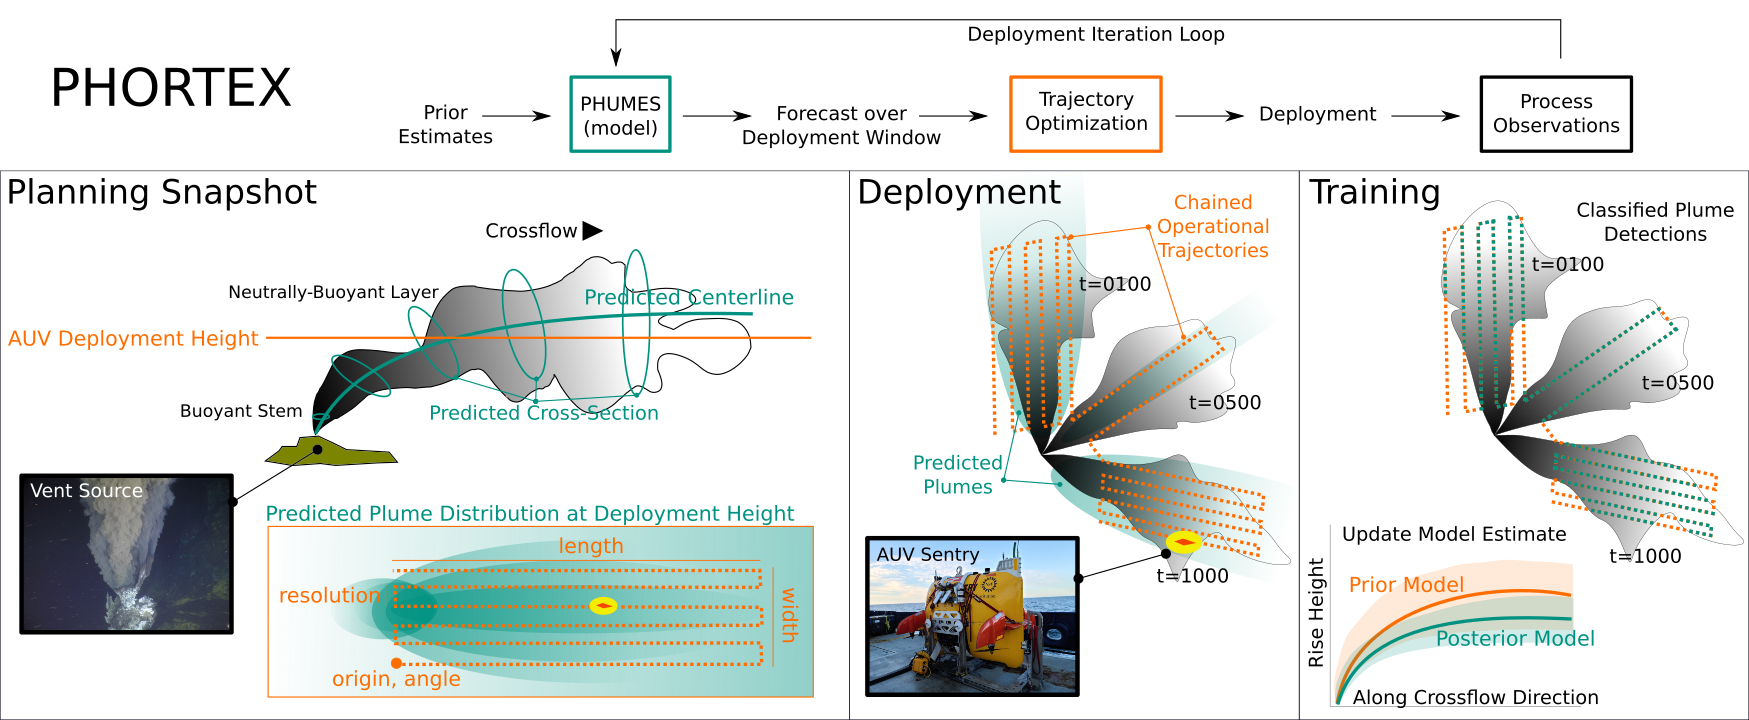
\includegraphics[width=\columnwidth]{figures/summary_intro_figure.png}
%     \caption{\textbf{An overview of \PHORTEX: \phortex.} Over the course of an expedition, an autonomous vehicle is deployed several times. In preparation for a deployment, the belief model \PHUMES: \phumes is used to generate a probabilistic forecast of the target spatiotemporal distribution. \PHUMES can be seeded with prior information from scientific knowledge, data of opportunity from other deployed sensing equipment, or previous robot deployments. A trajectory optimizer is given the forecasts and modifies the parameters of a trajectory primitive. Several primitives are chained together to form a complete deployment trajectory. The robot is then deployed and executes the trajectory. Following a deployment, \emph{in situ} observations from multiple heterogeneous science sensors are collected from the robot and fused into a data product that can be used to train \PHUMES, and the deployment planning process iterates. Here, the task of hydrothermal plume charting with AUV \emph{Sentry} is illustrated. \PHUMES generates a forecast of temporally-evolving plume centerlines and cross-sections from estimates of vent characteristics and fluid crossflow (e.g., current) informed by measurements or prior distributions over these variables. For a given height that \emph{Sentry} can operate (and is constrained to operate for any given primitive), chains of uniform coverage lawnmowers are optimized (over parameters such as height, width, origin, and global angle) with respect to the plume forecast to intersect and track the plume over the course of a deployment window. Following a \emph{Sentry} deployment, observation locations are classified as binary plume detections from analysis of several science sensors. This product is then used to update the \PHUMES model of plume centerline and cross-section over time. The new \PHUMES model is then used to plan the next deployment of \Sentry.}
%     \label{fig:intro_summary}
% \end{figure}

% \section{Background}

% \subsection{Hydrothermal Plume Charting}
% % We build on a wealth of work that has primarily focused on localizing hydrothermal venting plume sources (e.g., \citealt{jakuba2007stochastic, mcgill2011robot, nakamura2013discovery, paduan2018discovery, mason2020evaluation, wang20203, kim2020discovery,ferri2010novel}) using a variety of equipment such as ship-based acoustics, towed instrument rosettes, remotely-operated vehicles (ROVs), human-occupied submersibles (HOVs), and autonomous underwater vehicles (AUVs). 

% We build on a wealth of work that has primarily focused on localizing hydrothermal venting plume sources (e.g., \citealt{jakuba2007stochastic, mcgill2011robot, nakamura2013discovery, paduan2018discovery, mason2020evaluation, wang20203, kim2020discovery,ferri2010novel}). Generally, vent localization approaches use detections of anomalous water masses (as determined from \emph{in situ} sensors) in the water column to constrain the location of a seafloor vent. Specialized seafloor equipment is subsequently deployed at the inferred venting site to e.g., estimate bulk chemical or nutrient flux from the vent or characterize the driving magmatic system underneath the crust. The localization methods can be fully offline, in which surveys by vehicles like \Sentry with no adaptive capacity are post-processed and vent locations are inferred from a single survey \citep{jakuba2007stochastic,nakamura2013discovery}, or they can be fully online, in which autonomous gliders with adaptive capabilities utilize e.g., gradient descent to seek a plume source \citep{wang20203}. In \cite{branch2020demonstration}, an autonomous glider tasked with localizing a vent source could adaptively chain uniform coverage trajectories together with increasingly fine resolution as the robot position converged on an estimated vent location while underway. We emulate this chaining methodology in our trajectory chaining scheme, however the selection of trajectories by \PHORTEX is done completely offline before AUV \Sentry is deployed. Indeed, it is notable that online strategies for hydrothermal plume hunting almost universally employ glider-type robot platforms, which are typically smaller, payload-limited, and less depth-capable than vehicles like \Sentry. 90\% of known vent fields are deeper than \SI{200}{\meter} in the ocean, and over 75\% are deeper than \SI{1000}{\meter} \citep{beaulieu2013authoritative}. Gliders widely accessible to the research community are typically not rated deeper than \SI{1000}{\meter}, which means that deep-sea research of the majority of vent sites is reliant on vehicles like \Sentry and demand advances in offline-suited planning techniques.

% We also draw on ``plume hunting'' research in robotics, which has been equivalently styled as odor mapping, odor localization, source localization, and source seeking. In these works, the ``source'' emits a substance (e.g., gas, radio, acoustic, odor) and through partial observations of the emitted substance, the source is discovered using techniques that can be divided broadly into biologically-inspired heuristic search (e.g., \citealt{reddy2022olfactory,chen2019odor}) or adaptive informative path planning (e.g., \citealt{salam2019adaptive}). Biological or heuristic techniques draw (varying-levels of) inspiration from animal or insect behavior in olfactory settings. Such techniques typically include gradient-based algorithms like chemotaxis \citep{morse1998robust}, or algorithms that directly mimic a particular animal \citep{edwards2001representing}. These techniques are typically reactive and myopic, although they have been demonstrated to be relatively robust in open-world settings. In contrast, adaptive informative path planning can be nonmyopic, and typically attempts to embed knowledge (either heuristically or rigorously) about flow-fields (i.e., advection and diffusion) to assist in plume localization. Such techniques also live on a spectrum, from algorithms that resemble biologically-inspired techniques like infotaxis \citep{vergassola2007infotaxis} to methods that use model order reduction techniques (like proper orthogonal decomposition) to encode complex numerical models (like the Navier-Stokes equations) into a belief model to better treat complex data \citep{peng2014dynamic}.


% \section{Discussion}
% \subsection{Temporal Resolution in \PHUMES Forecasts}
% % some comments related to this discretization scheme, as opposed to using a ``puff'' model or other system
% The \PHUMES forecast provides a sequence of time-averaged plume ``snapshots'' over which trajectories for a given dive can be planned. By virtue of using the analytical model presented in \cref{sec:phumes}, generating a series of snapshots requires discretizing over time in order to sample a crossflow magnitude and heading, with which the global coordinates of a plume can be computed. This strategy does not capture the effects of advection and mixing on pre-existing (i.e., persistent) plume fluids; the snapshot from $t=0$ does not influence the snapshot of $t=1$ because the persistence of plume fluids generated at $t=0$ are not modelled directly). For the purposes of plume charting in the neutrally-buoyant layer, it could be advantageous to have a more sophisticated model of plume-fluid persistence and/or finer-scale temporal resolution in order to better constrain the spatiotemporal coordinates of a particular observation. For this sophistication to be added, two key innovations would be necessary: a suitable analytical model and a suitable observation scheme.

% In settings in which modeling fluid persistence may be useful, a simple advection-diffusion model could be used on-top of the analytical model we use in this work to advect neutrally-buoyant fluids between time discretized snapshots. This would be a simple extension that would introduce another uncertain parameter---rate of diffusion---for inference. Another methodology to explore may be integrating other probabilistic tools to estimate unmodeled characteristics of an environment by the analytical model (e.g., learned ``closure'' terms). This may be particularly well-suited in online planning domains, in which forecasts from an analytical model could be used e.g., to set the prior of a GP, and then live observations could be incorporated in real time for course correction while actually underway. Rather than build upon the model we selected, adapting Guassian puff models \citep{ludwig1977simplification} for the deep-sea environment or deriving a minimal set of PDEs to include derivatives in time from full-state models like in \cite{lavelle2013turbulent} could be fruitful. In this case, to consider persistence requires additionally modeling non-conservative properties of a plume, such as biological nutrient consumption or particulate deposition. As designing analytical models of these phenomenon is an active area of research, it is obvious that working with domain experts to formulate the right physically-informed model for \PHUMES is critical.

% The observation scheme for a particular implementation has considerable impact on the sophistication of the inference that can be accomplished. In hydrothermal plume charting, there are heuristics for particular sensors that we employed to create a simplified binary data product; however a similar scheme could be used to develop a more continuous measure of the ``plume-quality'' of a particular water sample, or a learned sensor could be developed which could potentially create a more expressive data product. One of the challenges with environmental domains is the access to enough training data to create such learned sensors. But perhaps the larger challenge is simply the quality of the data available at large---much of the carbonate and other biogeochemical systems of environmental interest have either a limited or nonexistent selection of (\emph{in situ}) sensors available to measure them. Of the sensors that exist, particularly for deep-sea work, the time-response of gas sensors is on the order of half-an-hour or longer (in this work, we made use of experimental sensors in active development with faster response times suitable for mobile AUVs). As the sophistication of sensing equipment improves, so too will the inference abilities of decision-making systems like \PHORTEX.  

\section{Methodology}
\subsection{Trajectory Optimization for Path Planning with Fixed Primitives}
\label{sec:to}
Given the hydrothermal plume-charting POMDP model introduced in \cref{sec:problem} and the probabilistic plume predictions generated by \PHUMES, we next consider how to select trajectories for AUV \Sentry that will effectively map the spatiotemporal dynamics of the evolving plume.  We first define a specific planning problem by re-writing the POMDP value function, \cref{eq:value}, in terms of the elements of the hydrothermal POMDP; then, we introduce a sequence of approximations that allow the value function to be feasibly optimized to select high-reward actions.

In each deployment, the planner must select an action in the form of a chained lawnmower trajectory (\cref{fig:traj_opt}). A chained lawnmower is defined by the number, $n \in \Z^+$, of lawnmowers in the chain and the parameters of each individual lawnmower, $\theta_i \in \Theta$ for $i = 1, \dots, n$. These parameters include the height, width, resolution, origin, and orientation of the lawnmower and are sufficient to completely specify a lawnmower trajectory. We define the set $\Theta$ to enforce that the lawnmower trajectories are contained within a pre-defined, rectangular safe region and that each lawnmower obeys a time-based budget constraint. As previously mentioned, this constrained action set is dictated by the operational practices of AUV \Sentry; lawnmower trajectories result largely in \Sentry traveling in straight lines with few, intermittent turns, which is a beneficial paradigm for the navigational sensors used onboard (i.e., acoustic Doppler Velocity Logger (DVL), inertial sensors). Using lawnmower trajectories has the additional benefit of biasing the vehicle to collect spatially diverse datasets that scientists are accustomed to analyzing. 

\begin{figure}[h!]
    \centering
    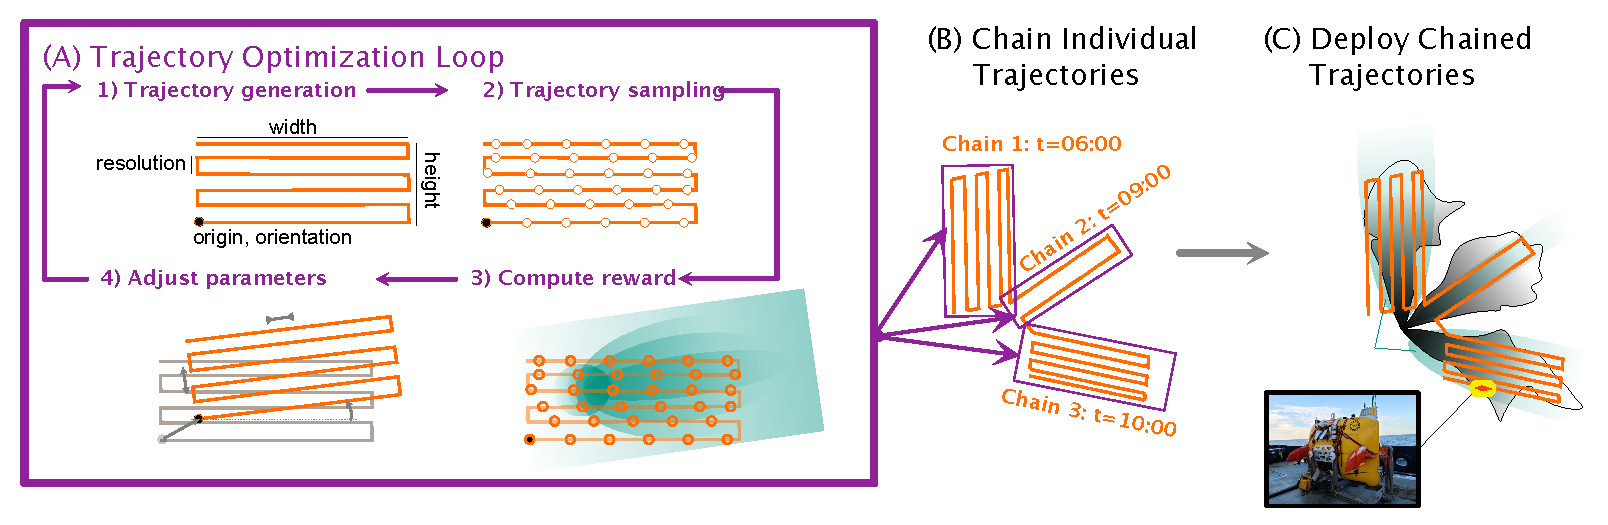
\includegraphics[width=1\columnwidth]{figures/trajectory_optimization.pdf}
    \caption{\textbf{Trajectory Optimization.} The trajectory optimizer leverages the \PHUMES simulator to select high-reward chains of parameterized lawnmower trajectories. (A) The optimization loop for a single lawnmower object, parameterized by height, width, resolution, origin, and orientation. To evaluate the reward of a specific parameter setting, 1) the lawnmower trajectory object is generated using the specified parameters; 2) the trajectory is uniformly sampled along its length to produce a set of sample locations; 3) the reward of those sample locations is computed using the \PHUMES model forecasts of the plume envelope; and 4) the lawnmower parameters are adjusted using gradient-based constrained optimization. (B) This core trajectory optimization loop is used to select parameters for each of a chain of $N$ lawnmowers executed at varying times during the deployment. (C) The chained trajectory is then operationally validated and deployed on AUV \Sentry to collect plume observations.}
    \label{fig:traj_opt}
\end{figure}

We can reformulate the general POMDP value function defined in \cref{eq:value} for the elements of the plume-charting POMDP:
\begin{align}
     V_h^{*}(b) &=  \max_{\{\theta_1, \dots, \theta_n, n \mid \theta_i \in \Theta, n \in \Z^+\}} \mathbb{E}_{[\x_{p}, \x_{c}, \x_{r}]^\top \sim b}[R([\x_{p}, \x_{c}, \x_{r}]^\top, \{\theta_1, \dots, \theta_n\})] \hspace{0.6cm} h \in [0, H-1],
    \label{eq:approx_value}
\end{align}
where each $\theta_i \in \Theta$ parameterizes one of the lawnmower trajectories in a length-$n$ sequence of chained trajectories, and $b$ is the planner's belief about the state of the plume, currents, and robot. In this equation, we see the first of two important planning approximations made by \PHORTEX. As mentioned in \cref{sec:problem}, we set the discount factor $\gamma$ to zero, removing the second, recursive portion of the value function. This approximation significantly reduces the complexity of approximating the POMDP value function, allowing each deployment to be optimized myopically. As deployments of AUV \Sentry are intermittent, time constrained, and start/end on a ship at arbitrary coordinates, the sequence of deployments are largely de-coupled; decisions made in one deployment have very little impact on the achievable reward of the next.
%Practically, this approximation only slightly compromises planner performance. Deployments of AUV \Sentry are constrained to start and end at the static location of the ship and the duration of each deployment is fixed by the operational constraints of the scientific expedition. This result of these operational constraints is that sequential deployments are largely de-coupled: decisions make in a deployment have very little impact on the achievable reward of the next deployment. 

Solving \cref{eq:approx_value} still involves selecting the number of chains $n$ and the joint optimization of all $n$ lawnmower trajectories in the chain. For a standard parameterization of a lawnmower (height, width, resolution, origin, orientation), this results in a challenging high-dimensional, non-convex, constrained optimization problem in which the dimensionality of the optimization problem changes with the number of lawnmowers selected in the chain. In a typical 15-hour deployment of AUV \Sentry that uses $n=15$, one-hour chained lawnmowers, this results in a 90-dimensional, non-convex joint optimization problem, which must then further be optimized over the number of lawnmowers $n$. Optimization is additionally complicated because evaluating the reward function is computationally expensive, requiring \PHUMES to produce a prediction of plume probability for the locations sampled by a given lawnmower, and by a lack of analytical gradients for the reward function with respect to the lawnmower parameters (gradients are instead computed numerically). 

To simplify the planning problem further to address chaining optimization, we make a second approximation. We assume that the number of chained lawnmowers is given, i.e., $n=N$, and decompose the joint optimization of all chains in a trajectory into $N$-independent optimization problems. This approximation allows us to break a high-dimensional, joint optimization problem into a sequence of much lower-dimensional optimization problems, and is a reasonable approximation if the travel cost between subsequent lawnmowers is not significant. 

The final \PHORTEX value function, with the two approximations we described, is given by the following:
\begin{align}
     V_h^{*}(b) &\approx  \max_{\theta_1 \in \Theta} \dots \max_{\theta_N\in \Theta} \mathbb{E}_{[\x_{p}, \x_{c}, \x_{r}]^\top \sim b}[R([\x_{p}, \x_{c}, \x_{r}]^\top, \{\theta_1, \dots, \theta_N\})] \hspace{0.6cm} h \in [0, H-1].
    \label{eq:approx2_value}
\end{align}
We solve \cref{eq:approx2_value}, which defines multiple, independent, non-convex, constrained optimization problems, using the trust-constrained method in the \texttt{scipy} optimization library for a fixed number of iterations \autocite{conn2000trust}. To evaluate the reward function $R([\x_{p}, \x_{c}, \x_{r}]^\top, \{\theta_1, \dots, \theta_N\})$, we define a trajectory sampler operator $\G: \Theta \to \R^{3 \times k}$ that takes a trajectory parameter vector as input and produces a set of locations in $\R^3$ that will be sampled when the robot executes the trajectory, where $k$ is the number of sampled points. In practice, our trajectory sampler $\G$ produces the lawnmower specified by $\theta$ and then subsamples uniformly along its length with a fixed spacing. These sample points can then be compared with the plume forecast $\mathbf{W}$ produced by \PHUMES to count the number of sample points that are contained within the inferred plume.


\subsection{At Sea Operations}
\PHORTEX was used to enable deployment-by-deployment autonomy during field operations with AUV \emph{Sentry} that fit within the typical workflow of operations at sea (\cref{fig:at_sea_ops}). Functionally, the trajectories planned with \PHORTEX were provided to the \Sentry engineering team for extensive safety validation prior to each deployment. If approved by the \Sentry team, the chief scientist, and captain of the vessel, the trajectories were downloaded into the \Sentry mission planning software as static waypoints. This confirmation process required a lead time of approximately 6 hrs before a scheduled deployment, and 12-18 hrs were available between deployments to mechanically service \Sentry and recharge batteries. The ability of \PHORTEX to produce viable trajectories from data within the first 6 hrs that \Sentry was on-deck following a recovery was critical for keeping this strict timeline. Given the long lead time between trajectory design and \Sentry deployment, there were many opportunities for the time of a deployment to change due to e.g., developments in weather, or other science/technology priorities. To be robust to these changes, we provided deployment plans that started several hours before and several hours after a given deployment time, and the \Sentry team truncated the plan at the appropriate points once a deployment time was known with certainty.

\begin{figure}[h!]
    \centering
    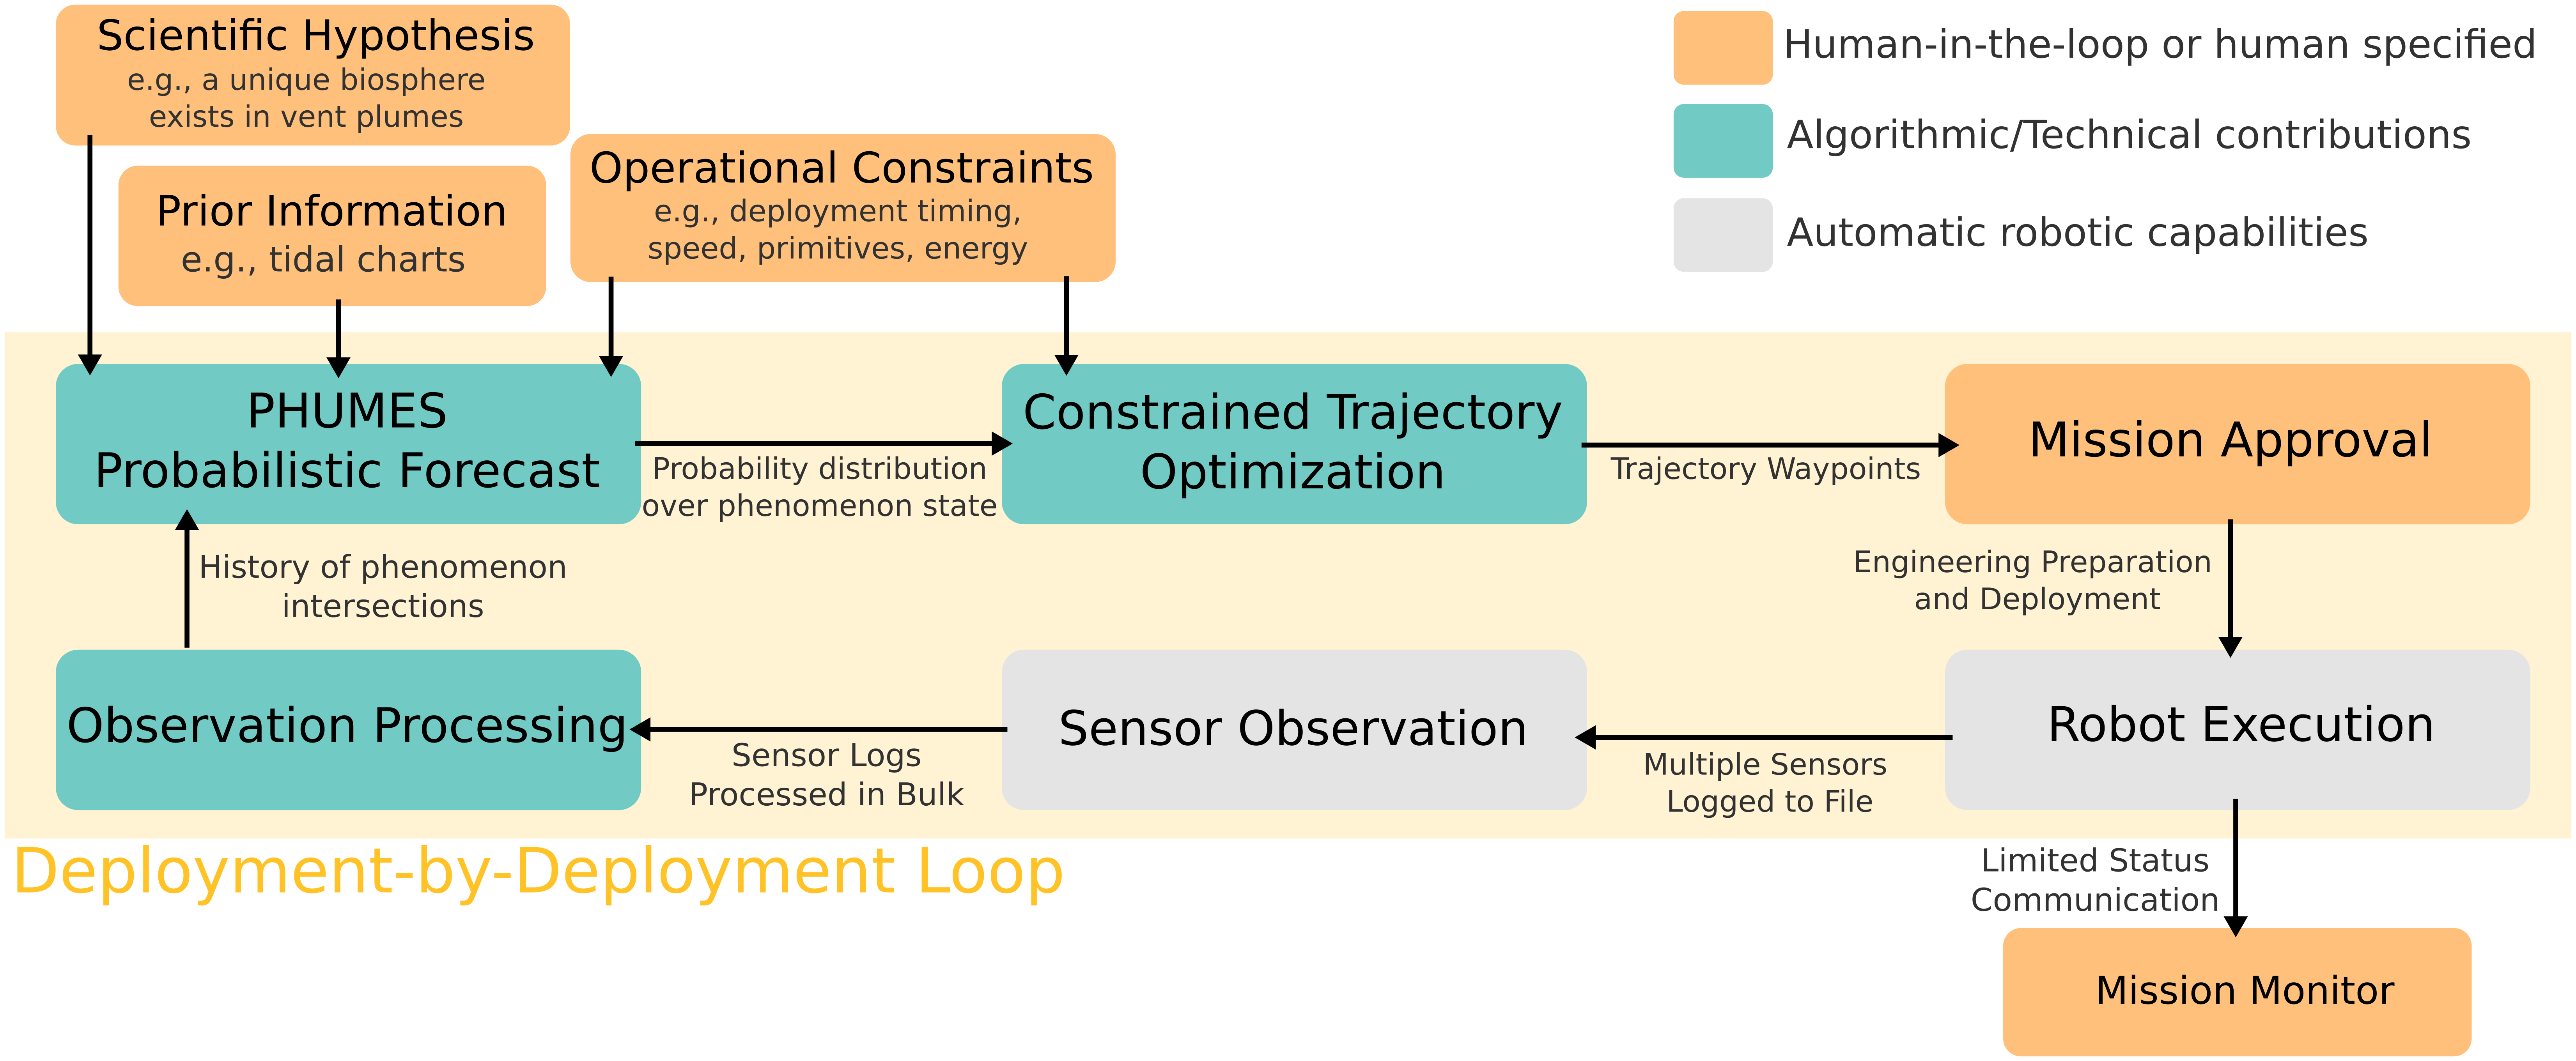
\includegraphics[width=0.9\columnwidth]{figures/deployment_loop.png}
    \caption{\textbf{The operational implementation of \PHORTEX at sea.} Integration of scientific knowledge, prior information, auxiliary sensor information, and operational constraints was done at the initialization of the \PHORTEX deployment-by-deployment loop. Every trajectory generated by \PHORTEX was checked by AUV \Sentry engineers and the science team before execution. \Sentry status was monitored with an external acoustic tracking system that monitored vehicle location, power, and performance while in acoustic range of the ship. Upon returning to deck, all science sensor observations were downloaded in bulk from the vehicle, and then ingested via our \PHORTEX system.}
    \label{fig:at_sea_ops}
\end{figure}

\section{Field Work and Simulation Results}
\subsection{Evaluation Metrics}
\label{sec:eval_metrics}
The scientific objective of \Sentry in the field trial is to collect observations of a deep-sea hydrothermal plume that have broad coverage in time and space, and thus are useful downstream for characterizing the space-time dynamics of the plume and other related phenomena (i.e., chemical flux, consumption). To evaluate the performance of \PHORTEX for deep-sea plume charting in both simulation and field trials in \cref{sec:experiments}, we introduce three key metrics that measure how well \Sentry collects such samples:
\begin{itemize}
    \item \textbf{Proportion of positive plume observations:} the number of observations collected in a dive that are classified as in-plume by the binary sensor model (\cref{sec:sensor_models}). This metric captures how effectively the robot targeted the plume during a deployment.
    \item \textbf{Spatial utilization:} the most distal plume detection and the ratio between the most distal plume detection and the longest distance that the robot traveled from the plume source. This metric captures the spatial coverage of the plume achieved by the robot and the spatial efficiency of the deployment. For example, if detections were made up to \SI{300}{\meter} away from the vent, but the robot traveled up to \SI{1}{\km} away, then the survey spent too much time outside of the detectable plume region and would not be as effective as a survey that only traveled \SI{200}{\meter} away but stayed well within the detectable plume range. 
    \item \textbf{Temporal utilization:} the proportion of hours in the dive with at least 10\% or more plume detections. This metric quantifies how effective the robot was at \emph{staying in} or \emph{revisiting} the plume over time. Given the long duration of these missions, it is important to use the entire mission window for the task at hand; moreover temporally diverse observations are of scientific interest.
\end{itemize}

\section{Experimental Results: Simulation and Field Trials}
\label{sec:experiments}

% Environment
\subsection{Simulation Experiments}
We investigate the performance of \PHORTEX in a simulated environment designed to replicate the field deployment closely. In the simulation, a point robot is tasked with collecting spatially and temporal diverse samples of an advecting plume. Each simulation is a three-dive series in which \PHORTEX starts with an uninformative prior over $\x_p$ and executes an initial naive survey (as would occur in a realistic field scenario), then iteratively updates \PHORTEX with collected observations and uses the the trajectory optimizer discussed in \cref{sec:to} to perform two more dives. We perform 10 three-dive simulations for each sampling/planning altitude of \SI{100}{\meter} and \SI{150}{\meter} in the same environment. Each single dive in the three-dive sequence is designed to be 12 hrs of simulated time, on a scale similar to the field deployment missions. 

In the simulator, the underlying analytical model in \PHUMES is used to generate a ground-truth environment that closely matches the conditions of the real-world vent using available data. The simulated environment has vent conditions of \SI{300}{\celsius}, 34.608 PSU salinity, \SI{0.8}{\meter\squared} orifice area, and \SI{0.6}{\meter\per\second} initial fluid velocity. The simulated environment sets the mixing coefficients to 0.15 and 0.2 for horizontal and vertical mixing, respectively. The current function sweeps a generated plume from due North to due East over the course of 12 hours of simulation time, and the magnitude cyclically varies with a beginning and end point of \SI{0.11}{\meter\per\second} and minimum at \SI{0.04}{\meter\per\second}. The generating current functions and snapshots of the true environment are provided in \cref{fig:sim_env}.

\begin{figure}[h!]
    \centering
    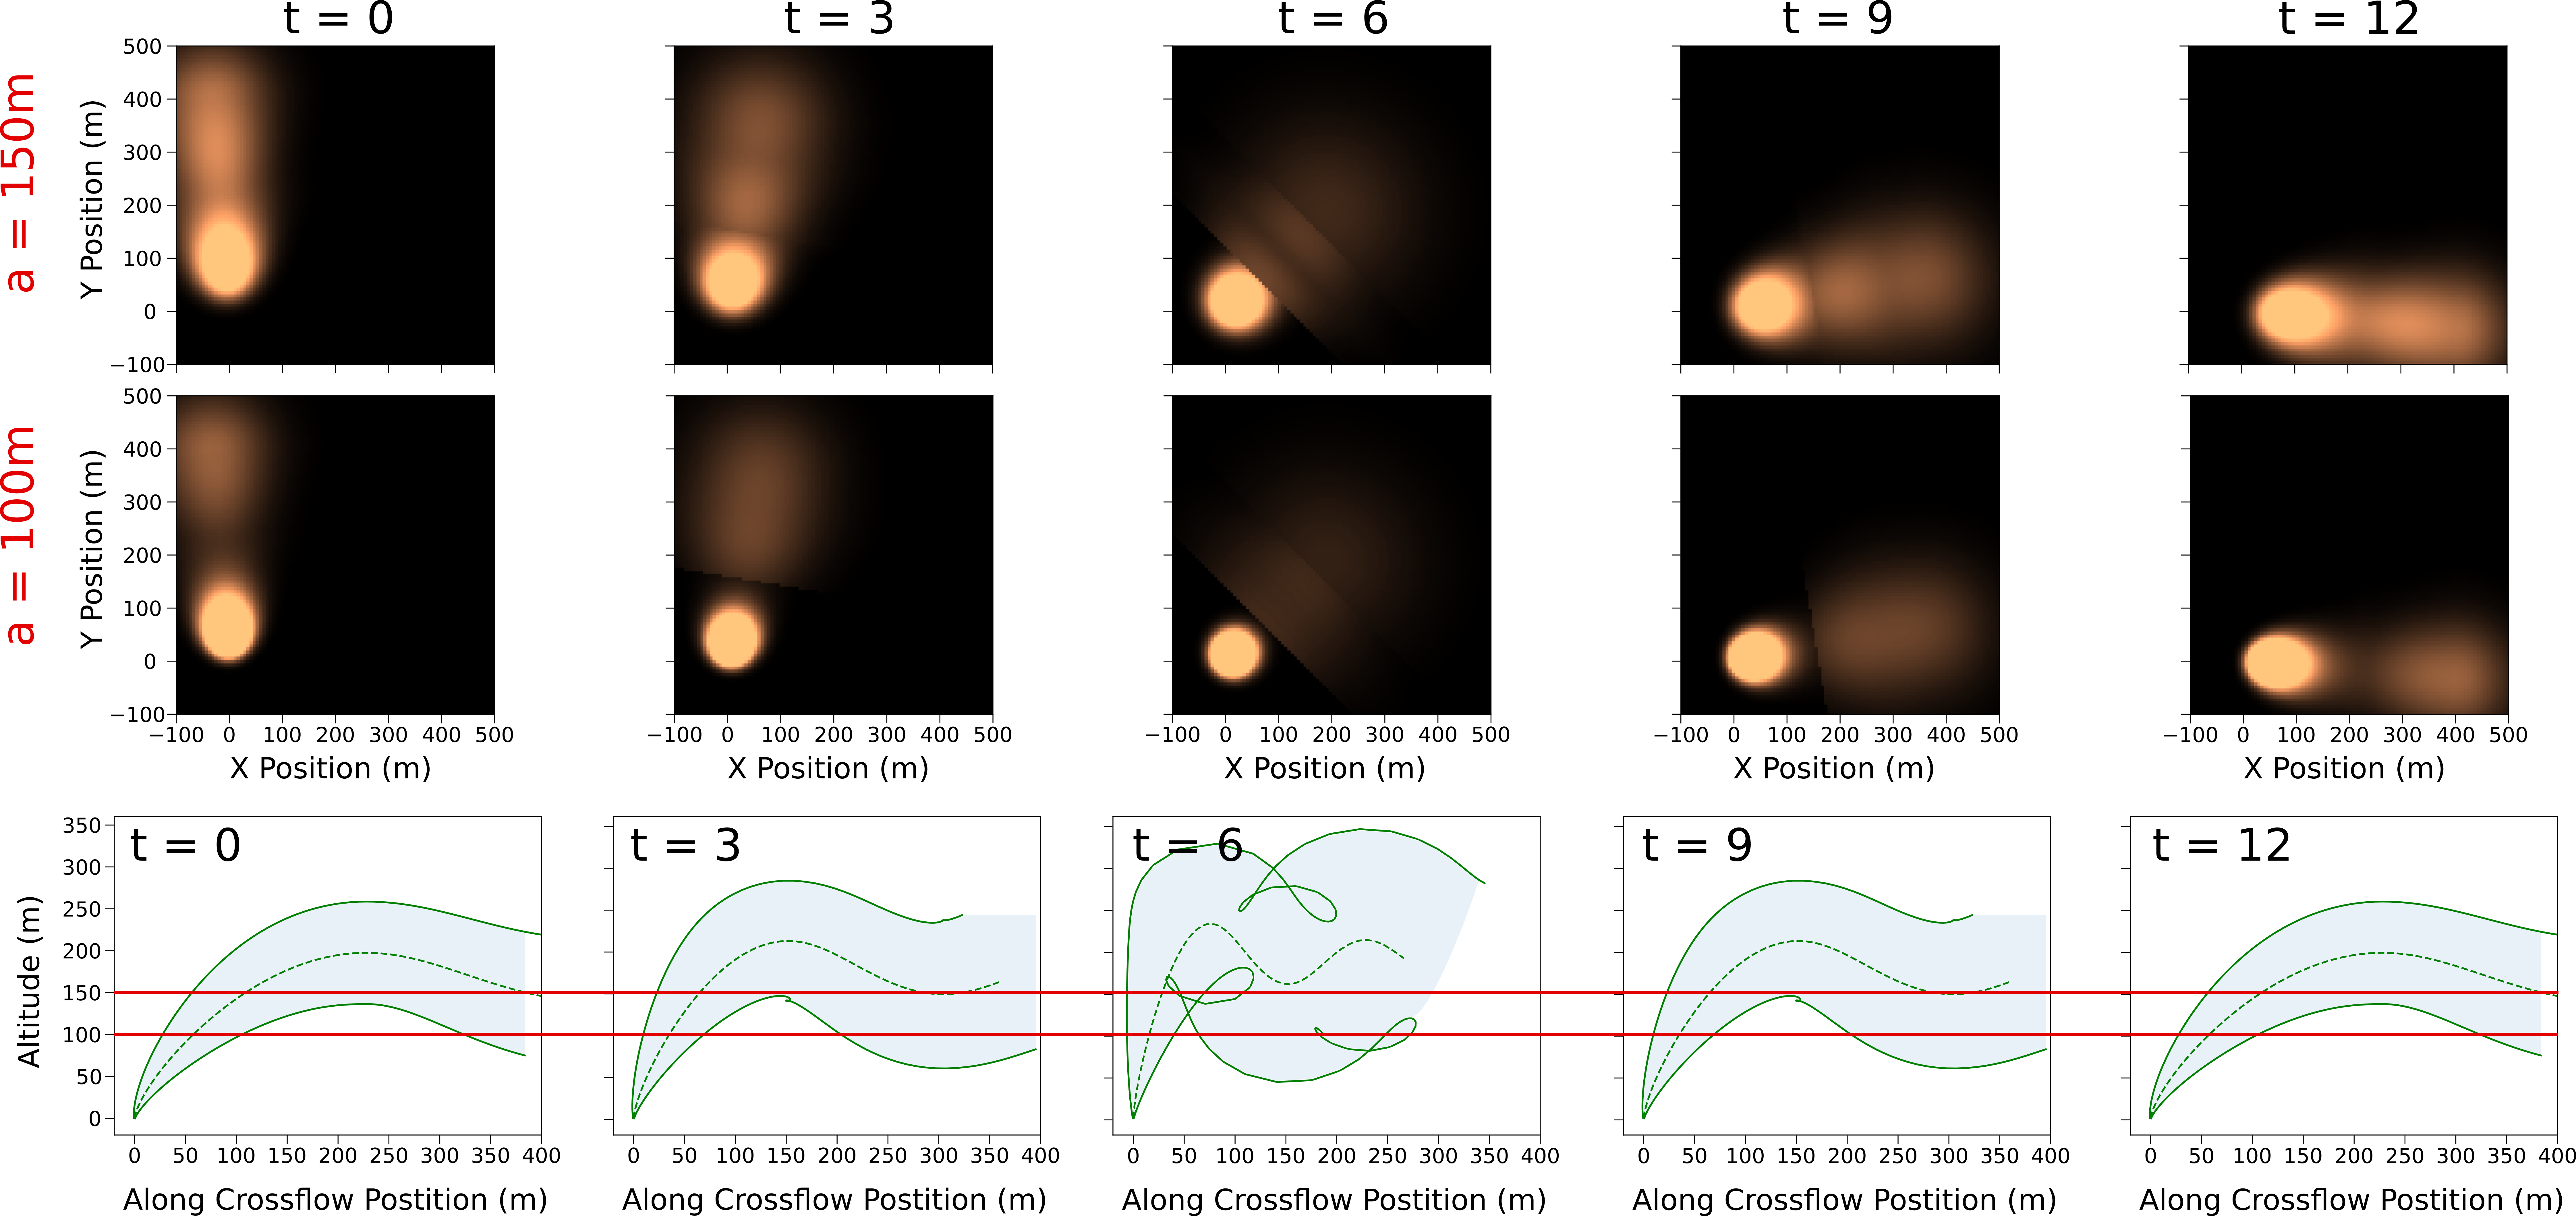
\includegraphics[width=1\columnwidth]{figures/sim_env.png}
    \caption{\textbf{Simulated field trial environment.} Generated environment for simulation trials at different snapshots for altitudes of \SI{100}{\meter} and \SI{150}{\meter}. As the current magnitude and heading changes, the plume expression changes shape and location over 12 hours. Plume intensity is shown in orange in the top plots. The bottom plots show a vertical cross-section of the plume envelope, along the crossflow direction, at different points in the tidal cycle, with the \SI{100}{\meter} and \SI{150}{\meter} horizontal planes marked.}
    \label{fig:sim_env}
\end{figure}

In these experiments, the \PHUMES model must estimate the vent area, vent fluid velocity, and both mixing coefficients from plume observation in the water column, starting with uninformative priors over each of these targets. A noisy current magnitude and heading function is provided to \PHUMES for use in the forecasting and updating step, as would typically be available from, for example, an auxiliary tiltmeter sensor (\cref{sec:aux_sensors}). For the \PHUMES update, 150 samples from an MH-MCMC chain are used to approximate the posterior distributions over the inference targets (this excludes an initial 50 samples of burn-in). In the first simulated dive, the robot executes a base-case uniformed lawnmower trajectory, placed to intersect the sweeping movement of the current. This trajectory is \SI{15}{\meter} in resolution, and covers a \SI{500}{\meter} by \SI{500}{\meter} area, with no rotation. For the second and third dives, trajectories are optimized using \PHORTEX for the 12-hour mission and consist of four, 3-hour long chained lawnmowers. Each lawnmower in the chain has a fixed resolution of \SI{10}{\meter}, and the height, width, origin, and orientation of each lawnmower are optimized to collect the most reward based on a plume forecast using the maximum \emph{a posteriori} (MAP) sample returned by the \PHUMES model for the four inference targets. The robot travels at approximately \SI{0.5}{\meter\per\second}, collecting binary observations every meter that is traveled. 

% Quality for this task is defined as collecting a high-proportion of in-plume samples over the course of a dive, revisiting a plume over the course of a dive, and collecting in-plume samples as far from the vent as the robot drives. 
\subsection{Simulation Experiments: Results}
\cref{fig:sim_traj_example} shows example planned trajectories and \cref{fig:sim_traj_perform} shows the distribution of each of the metrics of interest presented in \cref{sec:eval_metrics}---proportion in plume, spatial utilization, temporal utilization---for the three dives at each altitude tested in the trials. These results demonstrate that the \PHORTEX optimized trajectories significantly outperform the naive baseline, collecting over twice the proportion of samples in-plume, at least doubling the number of hours that the robot spends in a plume, and improving spatial utilization to nearly 100\% from 60-70\%. 

\begin{figure}[h!]
    \centering
    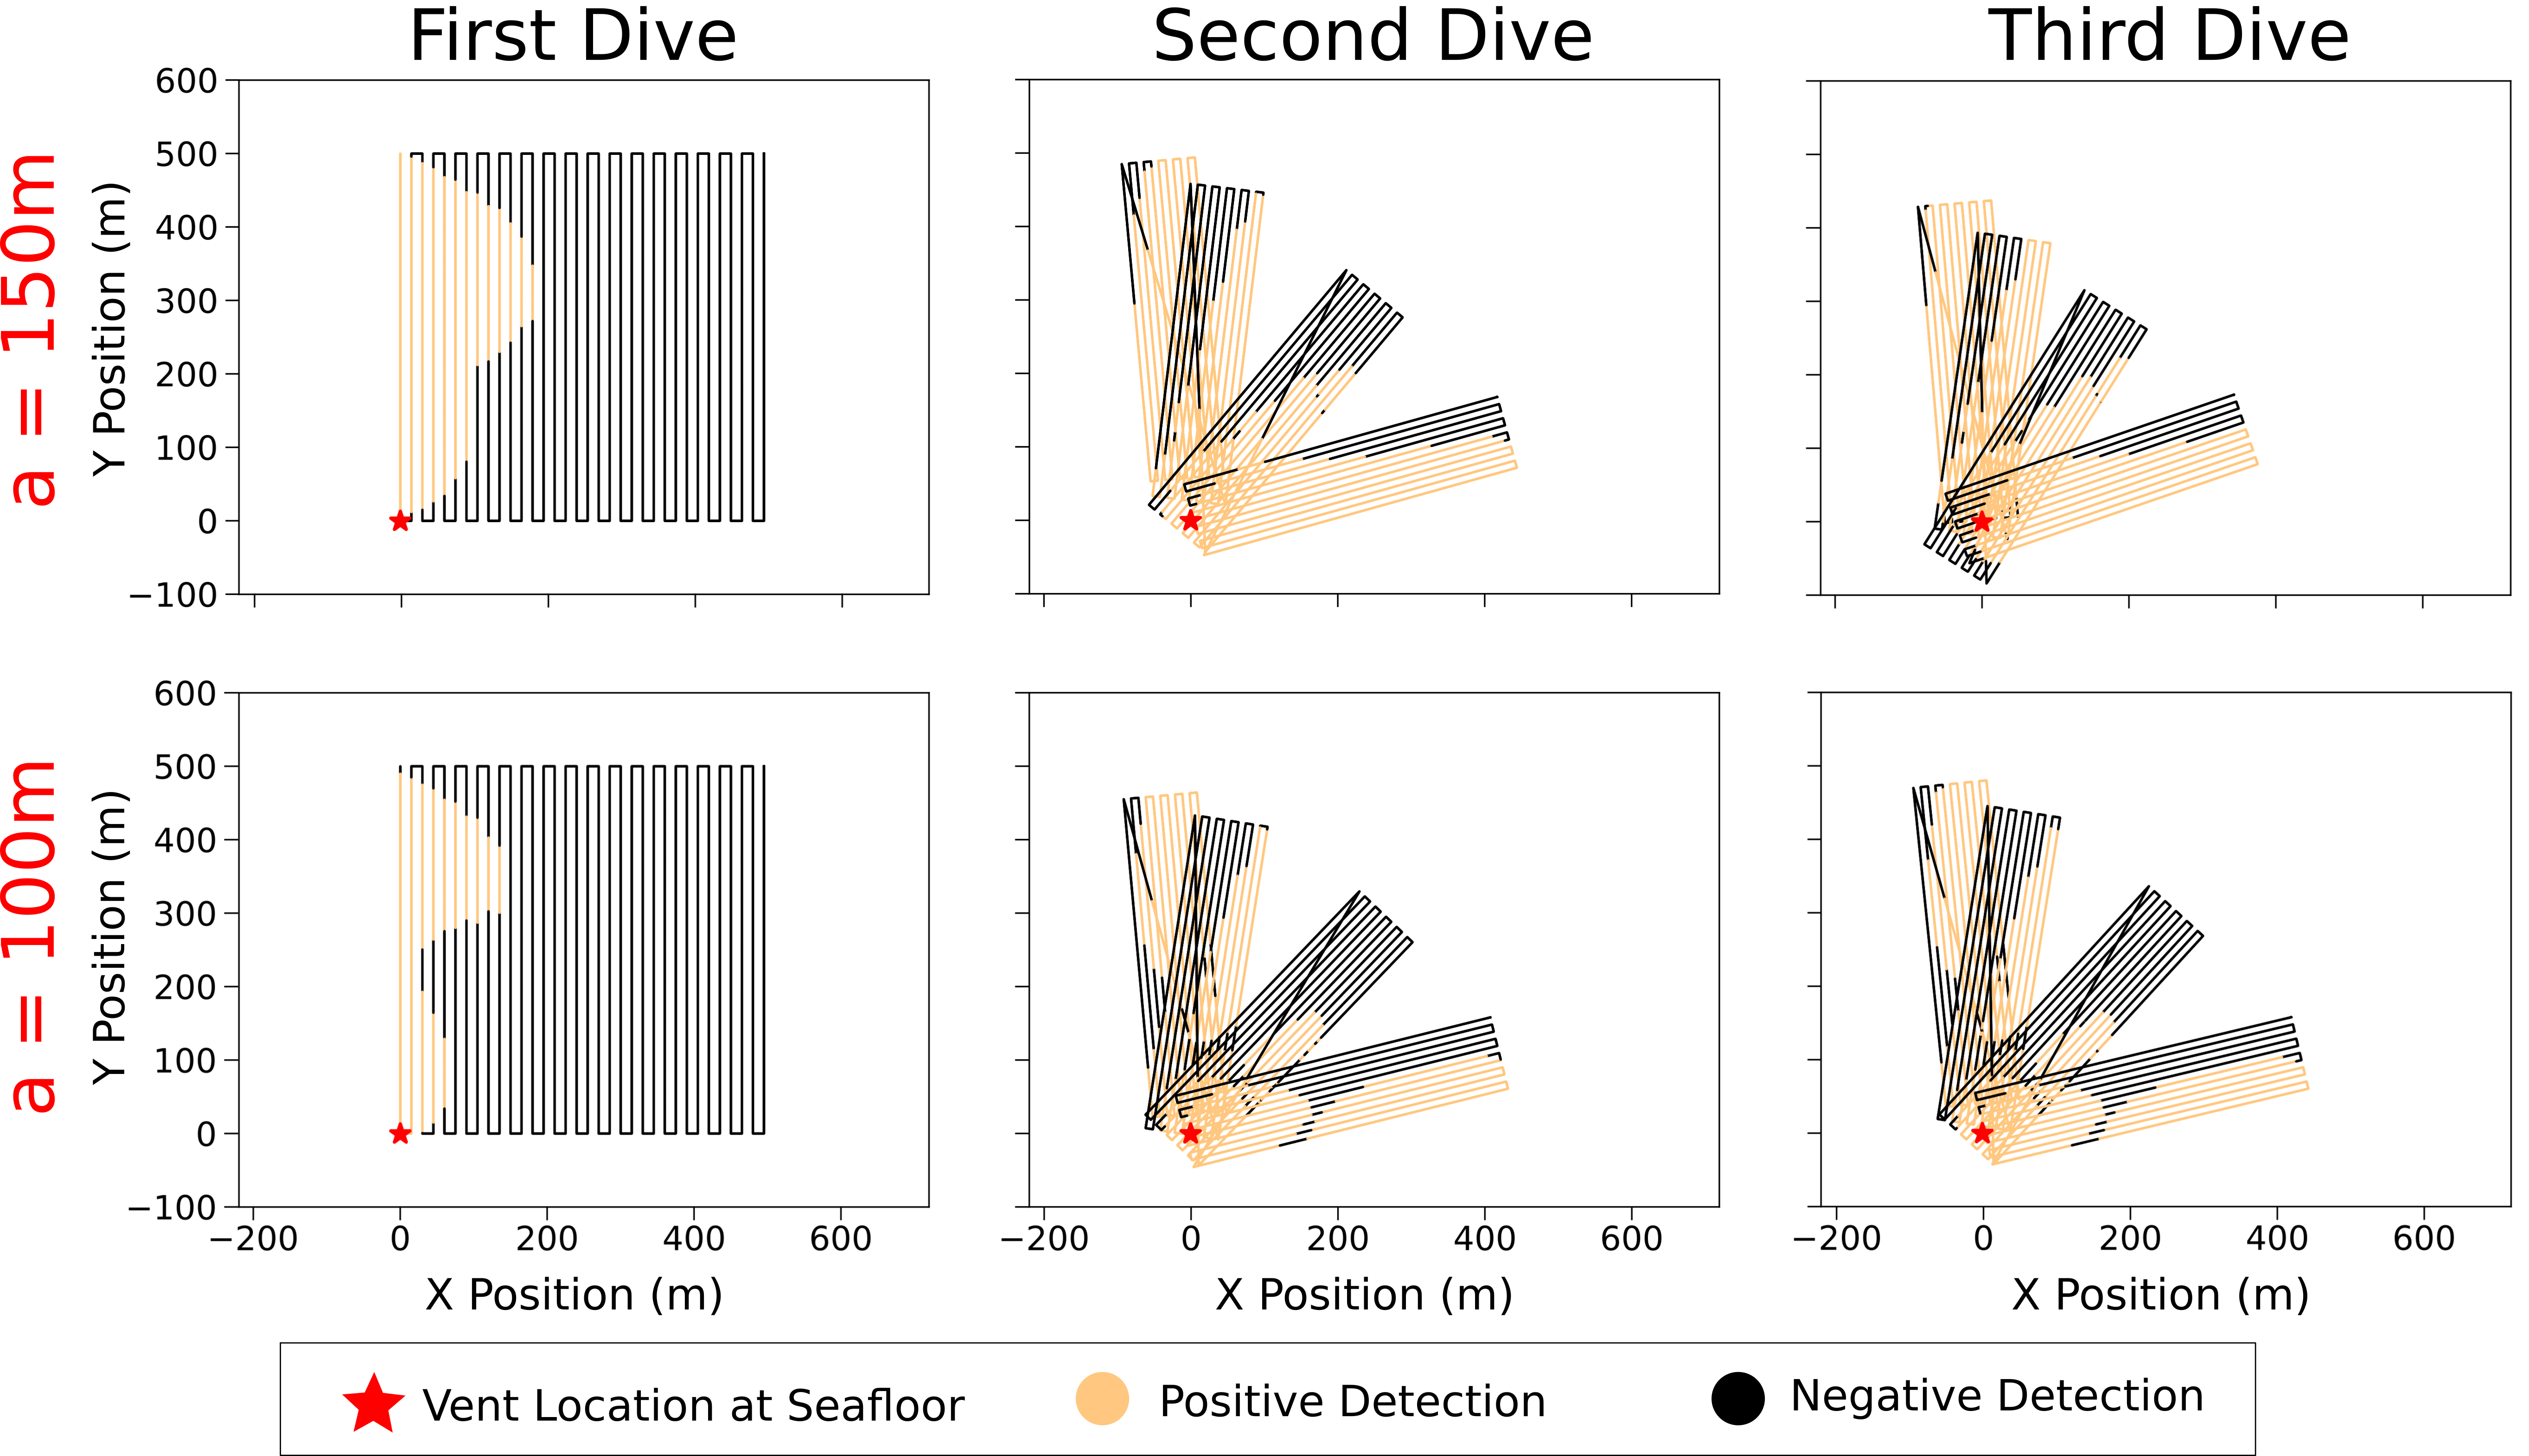
\includegraphics[width=0.85\columnwidth]{figures/sim_traj.png}
    \caption{\textbf{Naive and \PHORTEX-designed trajectories.} Trajectory examples for altitudes of \SI{100}{\meter} and \SI{150}{\meter}. The first dive is always a naive lawnmower; the second and third dive are \PHORTEX designed trajectories. \PHUMES is incrementally trained after each dive on the binary plume detections shown in this plot, which are sampled every meter traveled along the trajectory.}
    \label{fig:sim_traj_example}
\end{figure}

\begin{figure}[h!]
    \centering
    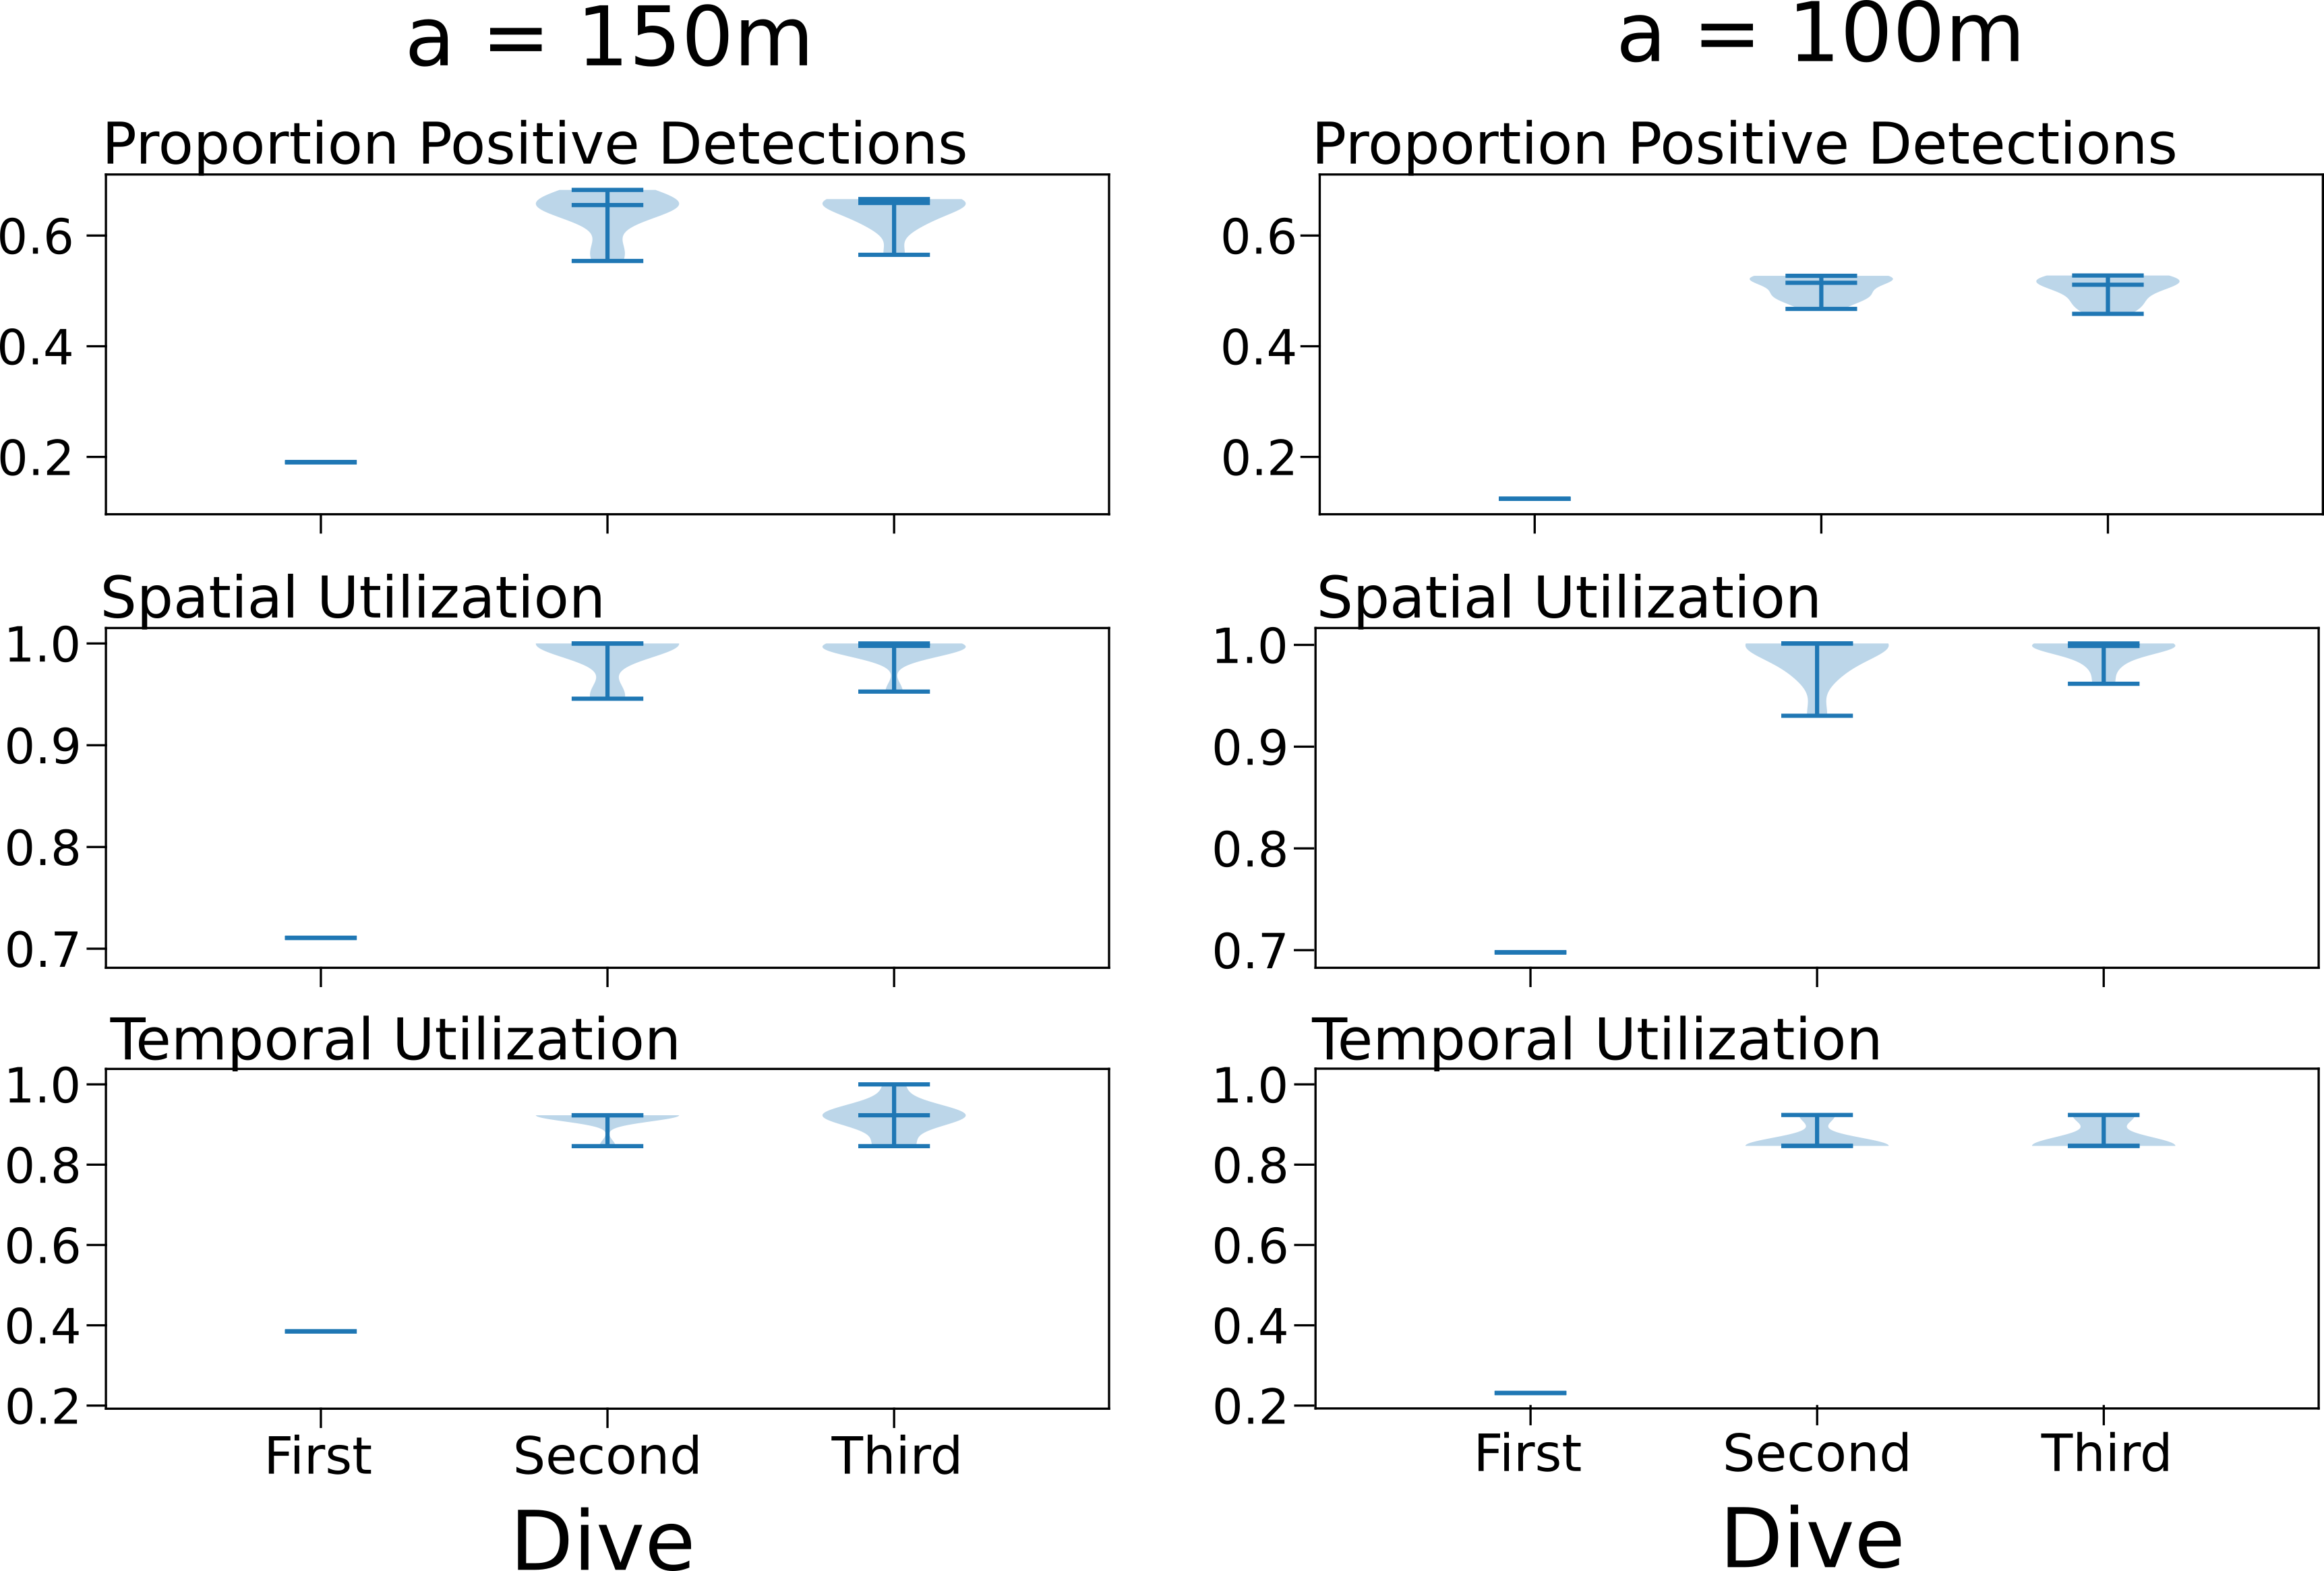
\includegraphics[width=0.75\columnwidth]{figures/sim_traj_performance.png}
    \caption{\textbf{Evaluation of the \PHORTEX trajectories.} The three-dive sequence, consisting of a naive lawnmower followed by two rounds of \PHUMES model training and \PHORTEX trajectory optimization, are evaluated for proportion of positive plume detections, spatial utilization, and temporal utilization (\cref{sec:eval_metrics}). The \PHORTEX-designed dives show a clear improvement in all three metrics, gathering more spatially and temporally diverse observations of the dynamic hydrothermal plume. Iterative rounds of \PHORTEX model-training and trajectory optimization continue to collect a high proportion of scientifically valuable observations.}
    \label{fig:sim_traj_perform}
\end{figure}


\paragraph{\PHUMES Model Validation}
The performance of \PHORTEX stays consistently high in the second and third dives, suggesting that \PHUMES quickly learns a sufficient model for planning from the small number of samples collected by the naive trajectories. To further understand the model learned by \PHUMES, we first qualitatively inspect the models learned by \PHUMES in two exemplar trials with data collected at \SI{100}{\meter} and \SI{150}{\meter} altitude during the initial naive survey of the first dive, as presented in \cref{fig:sim_model}. In the naive survey, less than 20\% of all detections are positive detections, and all detections only occur in the first 3 hours of the 12 hour mission. At an altitude of \SI{100}{\meter}, the robot essentially ``skims'' the bottom of the neutrally-buoyant plume; at \SI{150}{\meter}, the robot is consistently within the range of the neutrally-buoyant plume. Despite these altitude differences models learned in this example show remarkably similar characteristics---a predicted centerline no more than \SI{25}{\meter} off from the true environment's centerline, and a width that nearly completely envelopes the true plume distribution, which is promising for the context of planning missions. This is in contrast with an illustrative sample from the uninformative prior, which can arbitrarily produce plume structures that are significantly different in form from the true generating environment. It is also worth noting that despite training data only being available for 3 hours of the 12 hour simulated dive, the predictive quality of the model learned forecasts to an unseen time (t=9hrs) remains high. This largely demonstrates the advantage of using an embedded dynamics model in order to generate predictions of the state space to unseen times.

\begin{figure}[h!]
    \centering
    \includegraphics[width=\columnwidth]{figures/sim_mod.png}
    \caption{\textbf{Illustration of model learning.} Snapshots of the true generating environment are compared with an arbitrary sample from the prior distribution over \PHUMES parameters and the learned models from data collected by naive lawnmowers in both \SI{100}{\meter} and \SI{150}{\meter} simulation trials. In these two exemplar experiments, model learning performance is comparable between the \PHUMES models trained on data from different altitudes. The learned model, in comparison to the baseline sample, demonstrates a lower neutrally buoyant stem height, and is wider, and better explaining the data collected at the two sampling heights. Snapshots at different times show that the learned parameters robustly predict future shapes of the plume, even when trained on partial data available from the naive lawnmowers.}
    \label{fig:sim_model}
\end{figure}

To the quantify performance of the plume forecast generated by the MAP parameter sample after each trial, we compute the intersection over area (IoA) and intersection over union (IoU) between the true environment and each of the learned models after the naive and first \PHORTEX designed dives (\cref{fig:sim_phumes_perform}). A set of 10 parameter samples from the uninformative priors over the inference targets are used to generate an initialization performance distribution to show the breadth of forecast quality before any training. IoA (or recall) provides a number from 0-1 that expresses how many samples in the learned model are shared with the true generating environment. This number does not penalize false positives in the model: a value of 1 implies that all points in the model are contained by the environment, and a 0 implies that there are no points contained in the true environment. IoU (or precision) also provides a number from 0-1 that now penalizes false positives: a value of 1 implies perfect alignment between the model and environment, and a 0 implies no alignment. The comparison of these numbers helps to contextualize the performance of model learning. 

In \cref{fig:sim_phumes_perform}, we see that the learned models have a narrower performance window than the baseline samples, and that they generally exhibit very high IoA (up to 1), and a higher IoU (up to 0.9) than the baseline models (up to 0.75). With a high IoA, we can be confident that the learned models are placing value in areas for which there is plume, and with a higher IoU, we can be confident that the structure of the predicted regions with high value align well with the true environment. Taken together, a very high IoA with medium to high IoU suggest that trajectories planned with the \PHORTEX-trained models are very likely to plan for and successfully execute intersections with the targeted plumes, which is advantageous for our scientific task. We do not see a degradation of performance with different observations available between dives, suggesting that from very little data (a single naive dive), we can train an immediately useful model. Additionally, we note that there is a distinct difference in the distribution shapes of IoA and IoU between the altitudes across these trials. In particular, training from samples at \SI{150}{\meter} appears to be more consistently highly performant (IoA mode is at or near 1; IoU distributions skew towards 0.8) than at the lower altitude, which has a more distributed performance characteristic (with IoA skewed just about 0.8, and IoU centered just above 0.6). This has interesting implications for choosing deployment altitudes in practical missions, within the constraints of robot abilities (for instance, AUV \Sentry cannot swim over a certain altitude and maintain good localization, thus constraining what parts of a plume may be accessible in field deployments). We leave as future work the finer scale characterization of informativeness of different plume regions for model recovery in scientific settings.


\begin{figure}[h!]
    \centering
    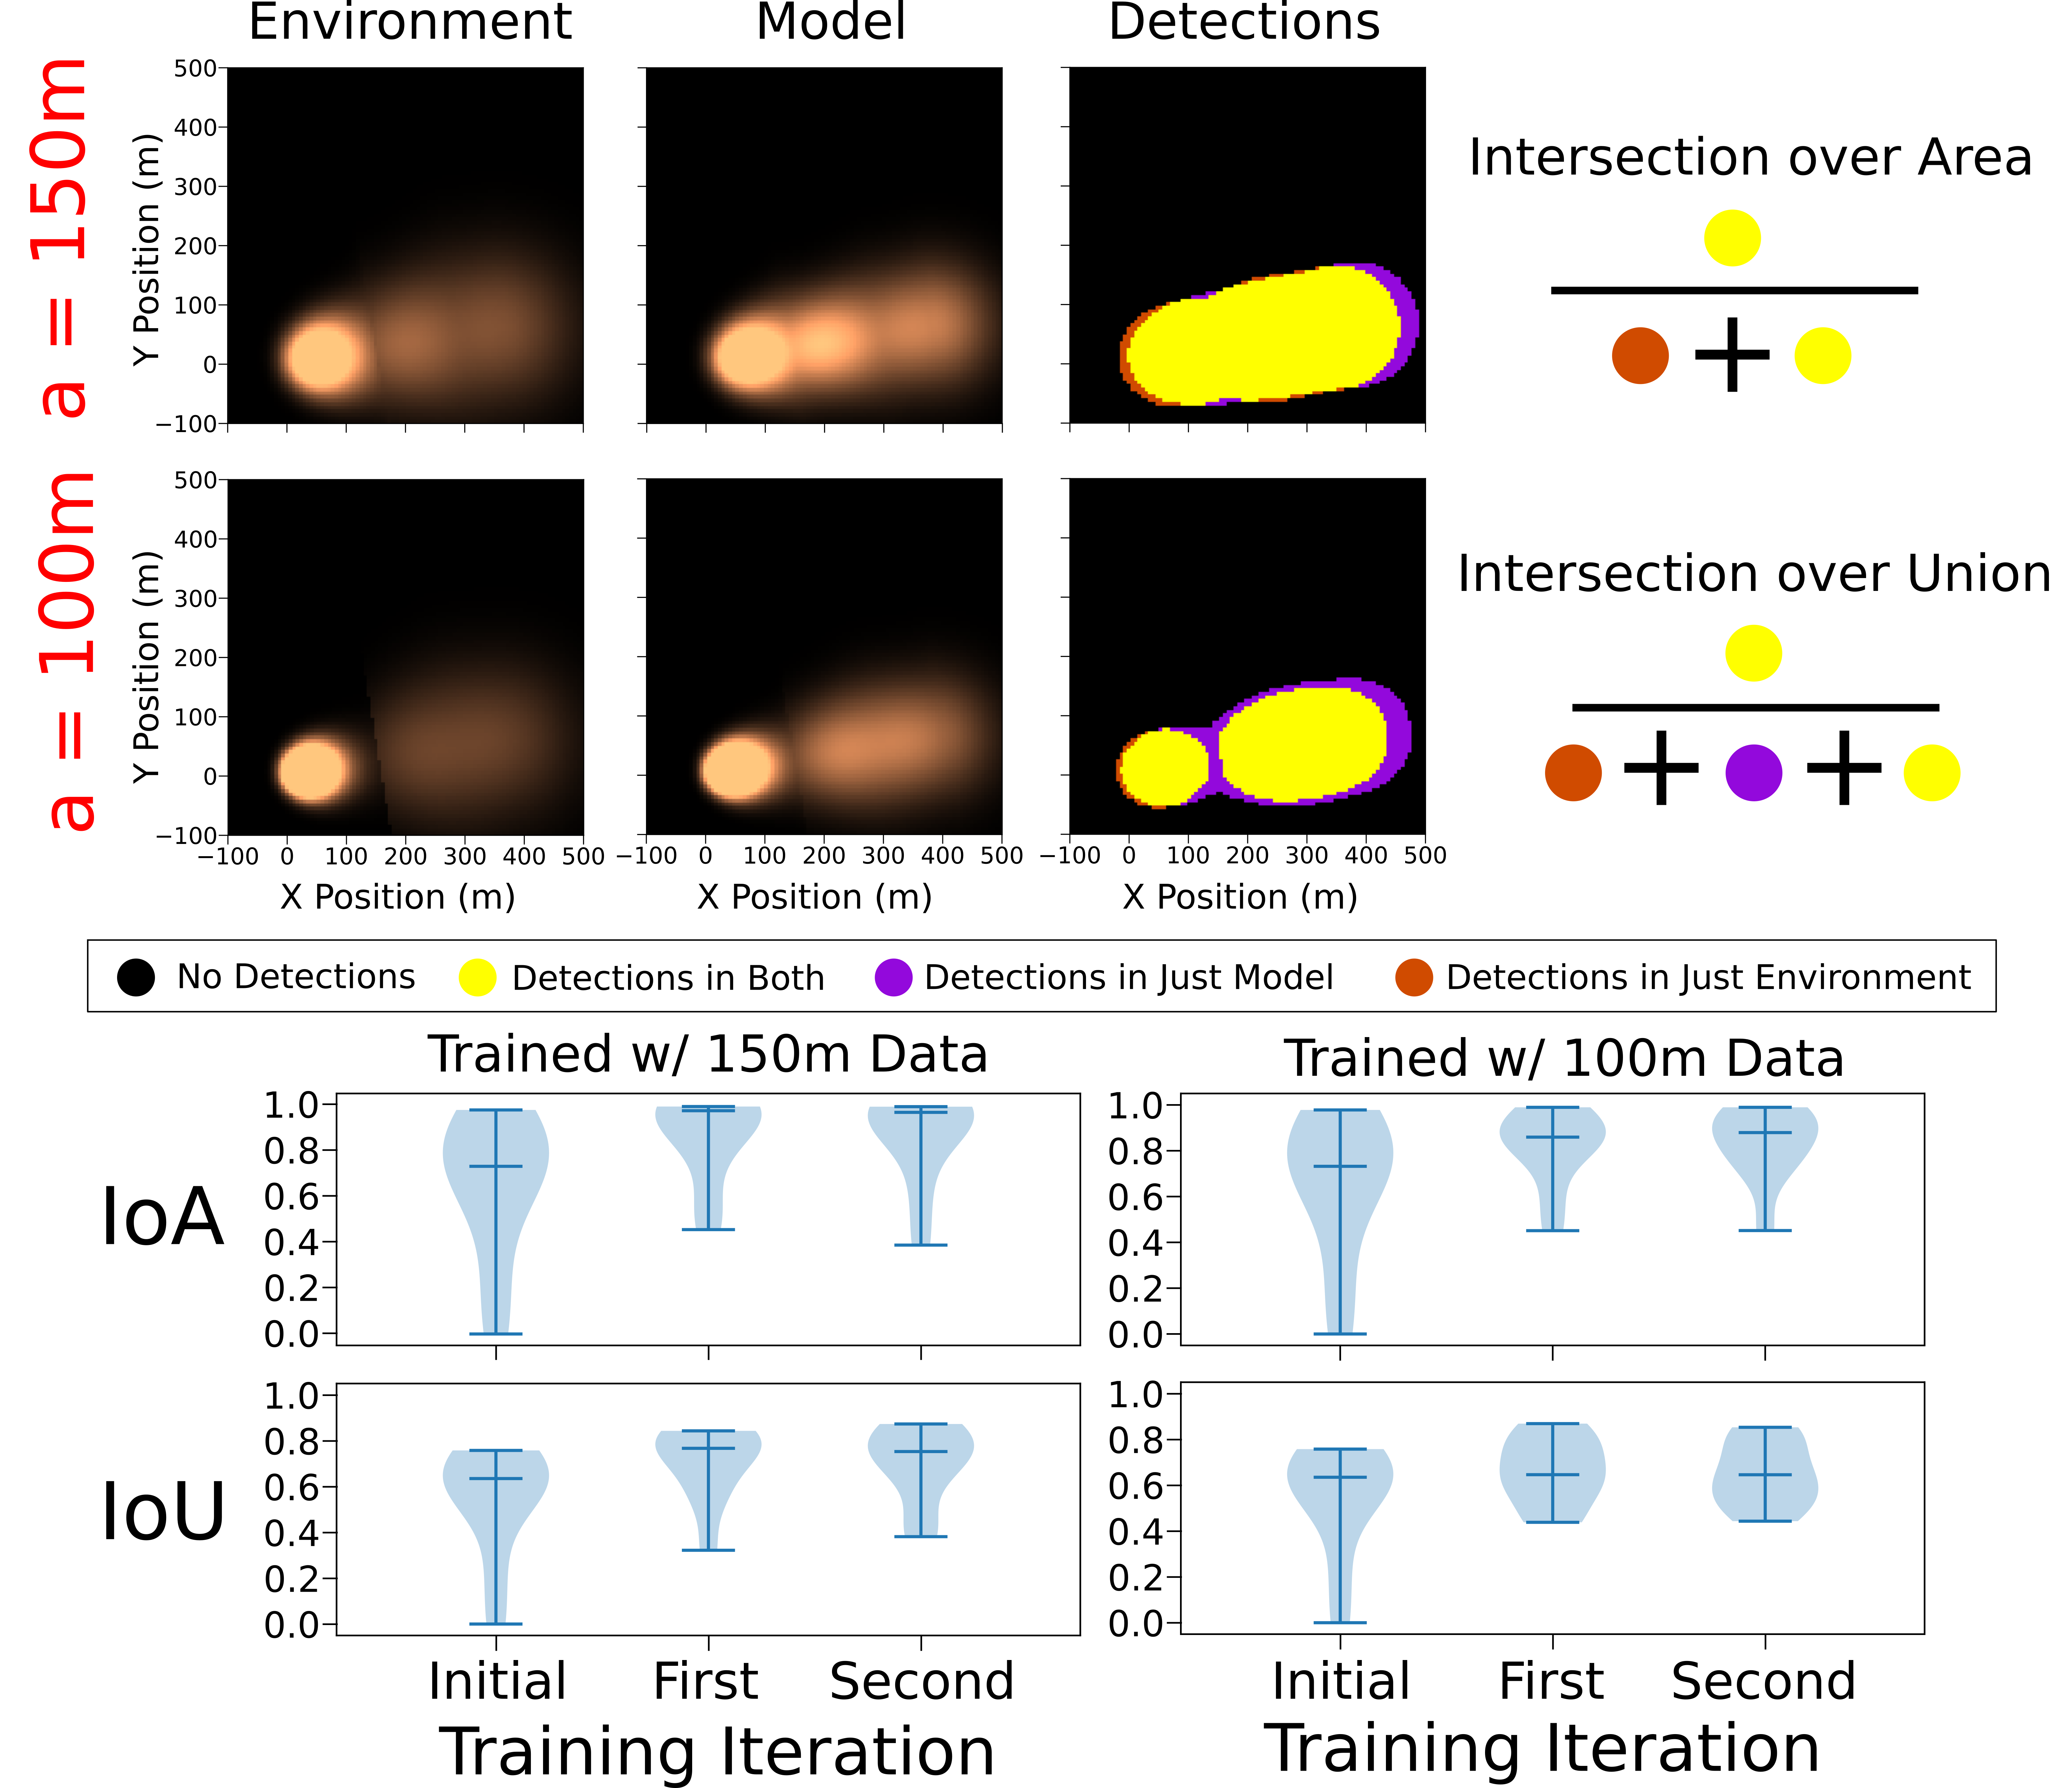
\includegraphics[width=0.9\columnwidth]{figures/sim_mod_performance.png}
    \caption{\textbf{Intersection over Area (IoA) and Intersection over Union (IoU) of trained models.} For each of trials trained from data at \SI{100}{\meter} and \SI{150}{\meter} altitudes, we compute the average IoA and IoU (using the method illustrated at the top) for a set of initial model samples (Initial), \PHUMES trained on the naive dive (First), and \PHUMES trained on the follow-up \PHORTEX-designed dive (Second). In general, we see the each of the iterative trained dives maintains similar performance; with high IoA and medium-to-high IoU that is consistently higher than initialized samples. Trials trained on data from \SI{150}{\meter} tend to have more performant model estimates (IoA near 1, IoU skewed above 0.8) compared to those trials trained on data from \SI{100}{\meter}.}
    \label{fig:sim_phumes_perform}
\end{figure}

% \begin{itemize}
%     \item We will first demonstrate \PHORTEX within the simulator we've created for generating plume funnels. We will show how \PHUMES converges to estimates of the true underlying distributions of initial conditions and parameter settings with and without noise. We will ideally show a graph that is RMSE of params versus mission iteration, and show a steep drop in error with steady improvement are iterations increase (fewer than 10 iterations will be graphed). 
%     \item We will additionally show performance on several key metrics, including reward versus iteration, total in-plume samples/accumulated reward under different model settings (e.g., number of samples in \PHUMES MCMC chain, prior uncertainty), and model mean and variance with each iteration. 
%     \item We will then show how sensitive trajectory optimization settings/chains are to collected reward, intending to show the advantage of using chains over a single highly-resolved lawnmower, at minimum.
%     \item If there is interest/time, we will then show how \PHORTEX performs in a numerically realistic simulator (as provided by our collaborator at University of Washington) and compute similar statistics as those indicated above. This addition would be used to demonstrate the complex real-time structure of plume snapshots, and show how the method generalizes to this setting. \VP{note that this is only if there is time; currently planning on only using the field results to demonstrate this, and may save simulation work for later tag-along conference/workshop paper}.
% \end{itemize}


\subsection{Field Trials with \PHORTEX at Sea}
In November 2021, \PHORTEX was used to design trajectories for AUV \Sentry at the Northern Guaymas Basin in the Gulf of California. Four deployments of AUV \Sentry were available to study the hydrothermal site. These deployments represent a planning spectrum, from fully human-designed surveys to fully \PHORTEX designed. We label the four deployments as follows:
\begin{itemize}
    \item \textbf{Dive H-Multi}: human designed, multi-task survey. This was the first deployment of \Sentry and the survey was designed to both attempt to find plume fluids and to bathymetrically map the local basin area (the map of which would be used as part of the safety check protocol for future deployments). This dive is representative of a standard nested strategy, in which progressively more targeted (finer resolution) surveys are used to study areas of interest. The dive was designed by a human expert who only had access to the approximate location of the target vent. The deployment lasted 21.3 hrs and collected 76,604 observations total.
    \item \textbf{Dive H-Plume}: human designed, plume-charting survey. This was the second deployment of \Sentry and the survey was hand-designed by the science party onboard the vessel to find and sample plume fluids. The science party had access to the performance of \Sentry in Dive H-Multi. The strategy was to sweep the basin above areas with known hydrothermal vents, and fly out into the basin in the direction that the plume fluids would be expected to advect. The deployment lasted 21 hrs and collected 75,430 observations total.
    \item \textbf{Dive HP-Plume}: hybrid human and \PHORTEX plume-charting survey. This was the third deployment of \Sentry and the survey consisted of trajectories designed by \PHORTEX trained by observations collected only in Dive H-Multi. Two of the trajectory primitives designed by \PHORTEX were replaced by ``naive'' lawnmowers placed over the known vent at two different times in the deployment. The deployment lasted 22.2 hrs and collected 79,792 observations total. Of these, 8.2 hrs and 29,438 observations were collected via the naive strategy.
    \item \textbf{Dive P-Plume}: \PHORTEX plume-charting survey. This was the fourth and last deployment of \Sentry. The survey was fully designed by \PHORTEX using observations only from Dive H-Multi, several days prior to this dive. The deployment lasted 9.9 hrs and collected 35,755 observations total. This deployment is notably much shorter than the other deployments due to increasing time constraints as the expedition was coming to a close. This deployment also used \Sentry in a ``depth-hold'' mode: whereas in all other dives \Sentry's depth followed the basin terrain, in this experiment the robot held an absolute depth.
\end{itemize}

\subsection{Field Trials with \PHORTEX at Sea: Results}
Using the metrics introduced in \cref{sec:eval_metrics}, we evaluate each of the four dives executed at sea to chart the space-time dynamics of a real hydrothermal plume as presented in \cref{tab:field_results} and visualized in \cref{fig:field_results}. Each dive took place at different times in the tidal cycle, on different days, and often at different altitudes in the water column, and thus the total plume samples available to collect during each dive is variable. With this in mind, we present and evaluate each dive quantitatively, and additionally qualitatively examine each as a case study for how different sampling paradigms perform in the real-world. There is no ground-truth available for the deep sea plume-charting problem; we evaluate each \Sentry dive assuming that the binary detections produced by the method in \cref{sec:sensor_models} are honest representations of the presence or absence of hydrothermally-derived fluids in the basin. 

The results of the field deployment in \cref{tab:field_results} demonstrate that \PHORTEX performs comparably to science expert-designed trajectories in the proportion of samples that are collected during dives, and importantly improves upon the spatial utilization (increasing both the range of the most distal plume detection and effectively utilizing of the entire explored range). This is most evident in the HP-Plume dive, in which the human designed portion is a naive lawnmower placed ``on top'' of the vent; the \PHORTEX-designed trajectory collects samples over twice as far from the plume source. Absolute temporal utilization is similar to human surveys; however the distribution of detections within the temporal utilization windows is improved --- for human surveys, detections tend to be ``bunched'' to either the first half (as in H-Plume) or second half (as in H-Multi). We see this most sharply in HP-Plume, in which 90\% of positive detections collected by the human-designed survey occurred only in the second of the two lawnmowers, from hours 20-23. In contrast, \PHORTEX designed trajectories collected detections more uniformly over the entire dive.  \cref{fig:field_results} shows the qualitative structure of each dive and showcases the diversity in the resulting datasets.

% Evaluating the efficacy of human- and \PHORTEX-designed trajectories in charting the space-time dynamics of a real-world hydrothermal plume is challenging. Unlike the simulation experiments, there is no ground-truth plume chart available and evaluating the counterfactual --- if \PHORTEX had gone here instead, how many more observations of the plume would have been collected? if we had used a naive planner instead of \PHORTEX for this deployment, how many fewer observations of the plumes would we have?--- is not straightforward. Due to operational constraints and the value of ship time, using an entire deployment of \Sentry to implement a lower-performing baseline is prohibitively wasteful; each deployment attempts to make the best use of available data to accomplish the task of plume charting.  In the remainder of the section, we evaluate each \Sentry dive using the metrics introduced in \cref{sec:eval_metrics}, assuming that the binary detections produced by the method in \cref{sec:sensor_models} are ground-truth detections and non-detections. 

% We look at several key metrics for each deployment: proportion of positive plume observations, utilization of spatial extent, and utilization of temporal dive window. The first metric, proportion of positive plume observations, is simply the number of observations collected in a dive that were classified as in-plume by the binary sensor model we describe in \cref{sec:sensor_models}. The second metric attempts to show how spatially effective the design of the survey was by first showing the absolute range that positive detections were made as a measure of distance from the chimney vent location and second showing how that range fit with the overall design of the survey. For example, if detections were made up to 300 m away from the vent, but the robot traveled up to 1 km away, then the survey spent too much time outside of the detectable plume region and would not be as effective as a survey that only traveled 200 m away but stayed well within the detectable plume range. Finally, the last metric is a measure of how effective the survey was at \emph{staying in} or \emph{revisiting} a plume over time. Given the duration of these missions, it is important to use the entire mission window for the task at hand; moreover temporally ``diverse'' observations are of scientific interest generally. We report the proportion of dive hours with at least 10\% or more positive detections.



\begin{table}[h!]
    \centering
    \begin{tabular}{c|c|c|c|c|c}
        Dive & Duration & Total Obs. & Prop. In-Plume & Spatial Util. & Temporal Util.  \\
        \hline
        H-Multi & 21.3 hrs & 76,604 & 22.3\% & \SI{300}{\meter} (19\%) & 9-17,20-21 (52\%) \\
        H-Plume & 21 hrs & 75,430 & 10.9\% & \SI{900}{\meter} (64\%) & 2,5-8,10-11,15-16 (43\%) \\
        \hline
        HP-Plume & 22.2 hrs & 79,792 & 41.8\% & \SI{600}{\meter} (100\%) & 1-3,5,7,11-23 (81\%) \\
        HP-Plume (H) & 8.2 hrs & 29,438 & 42.3\% & \SI{250}{\meter} (100\%) & 5,7,20-23 (75\%) \\
        HP-Plume (P) & 14 hrs & 50,354 & 41.5\% & \SI{600}{\meter} (100\%) &  1-3,11-20 (93\%)\\
        \hline
        P-Plume & 9.9 hrs & 35,755 & 12.8\% & \SI{450}{\meter} (100\%) & 1,5,8,9 (40\%)
    \end{tabular}
    \caption{\textbf{Per-dive statistics for field trials of \PHORTEX.} The spatial utilization is reported as both the most distal plume detection (measured from the plume origin) and the ratio of the most distal plume detection over the farthest distance that the robot traveled from the plume origin. Temporal utilization shows both which hours contain at least 10\% positive plume detection and what fraction of the total deployment duration contained such detections. The deployment HP-Plume is broken further into human designed (H) and \PHORTEX designed (P) portions for direct comparison.}
    \label{tab:field_results}
\end{table}

\begin{figure}[h!]
    \centering
    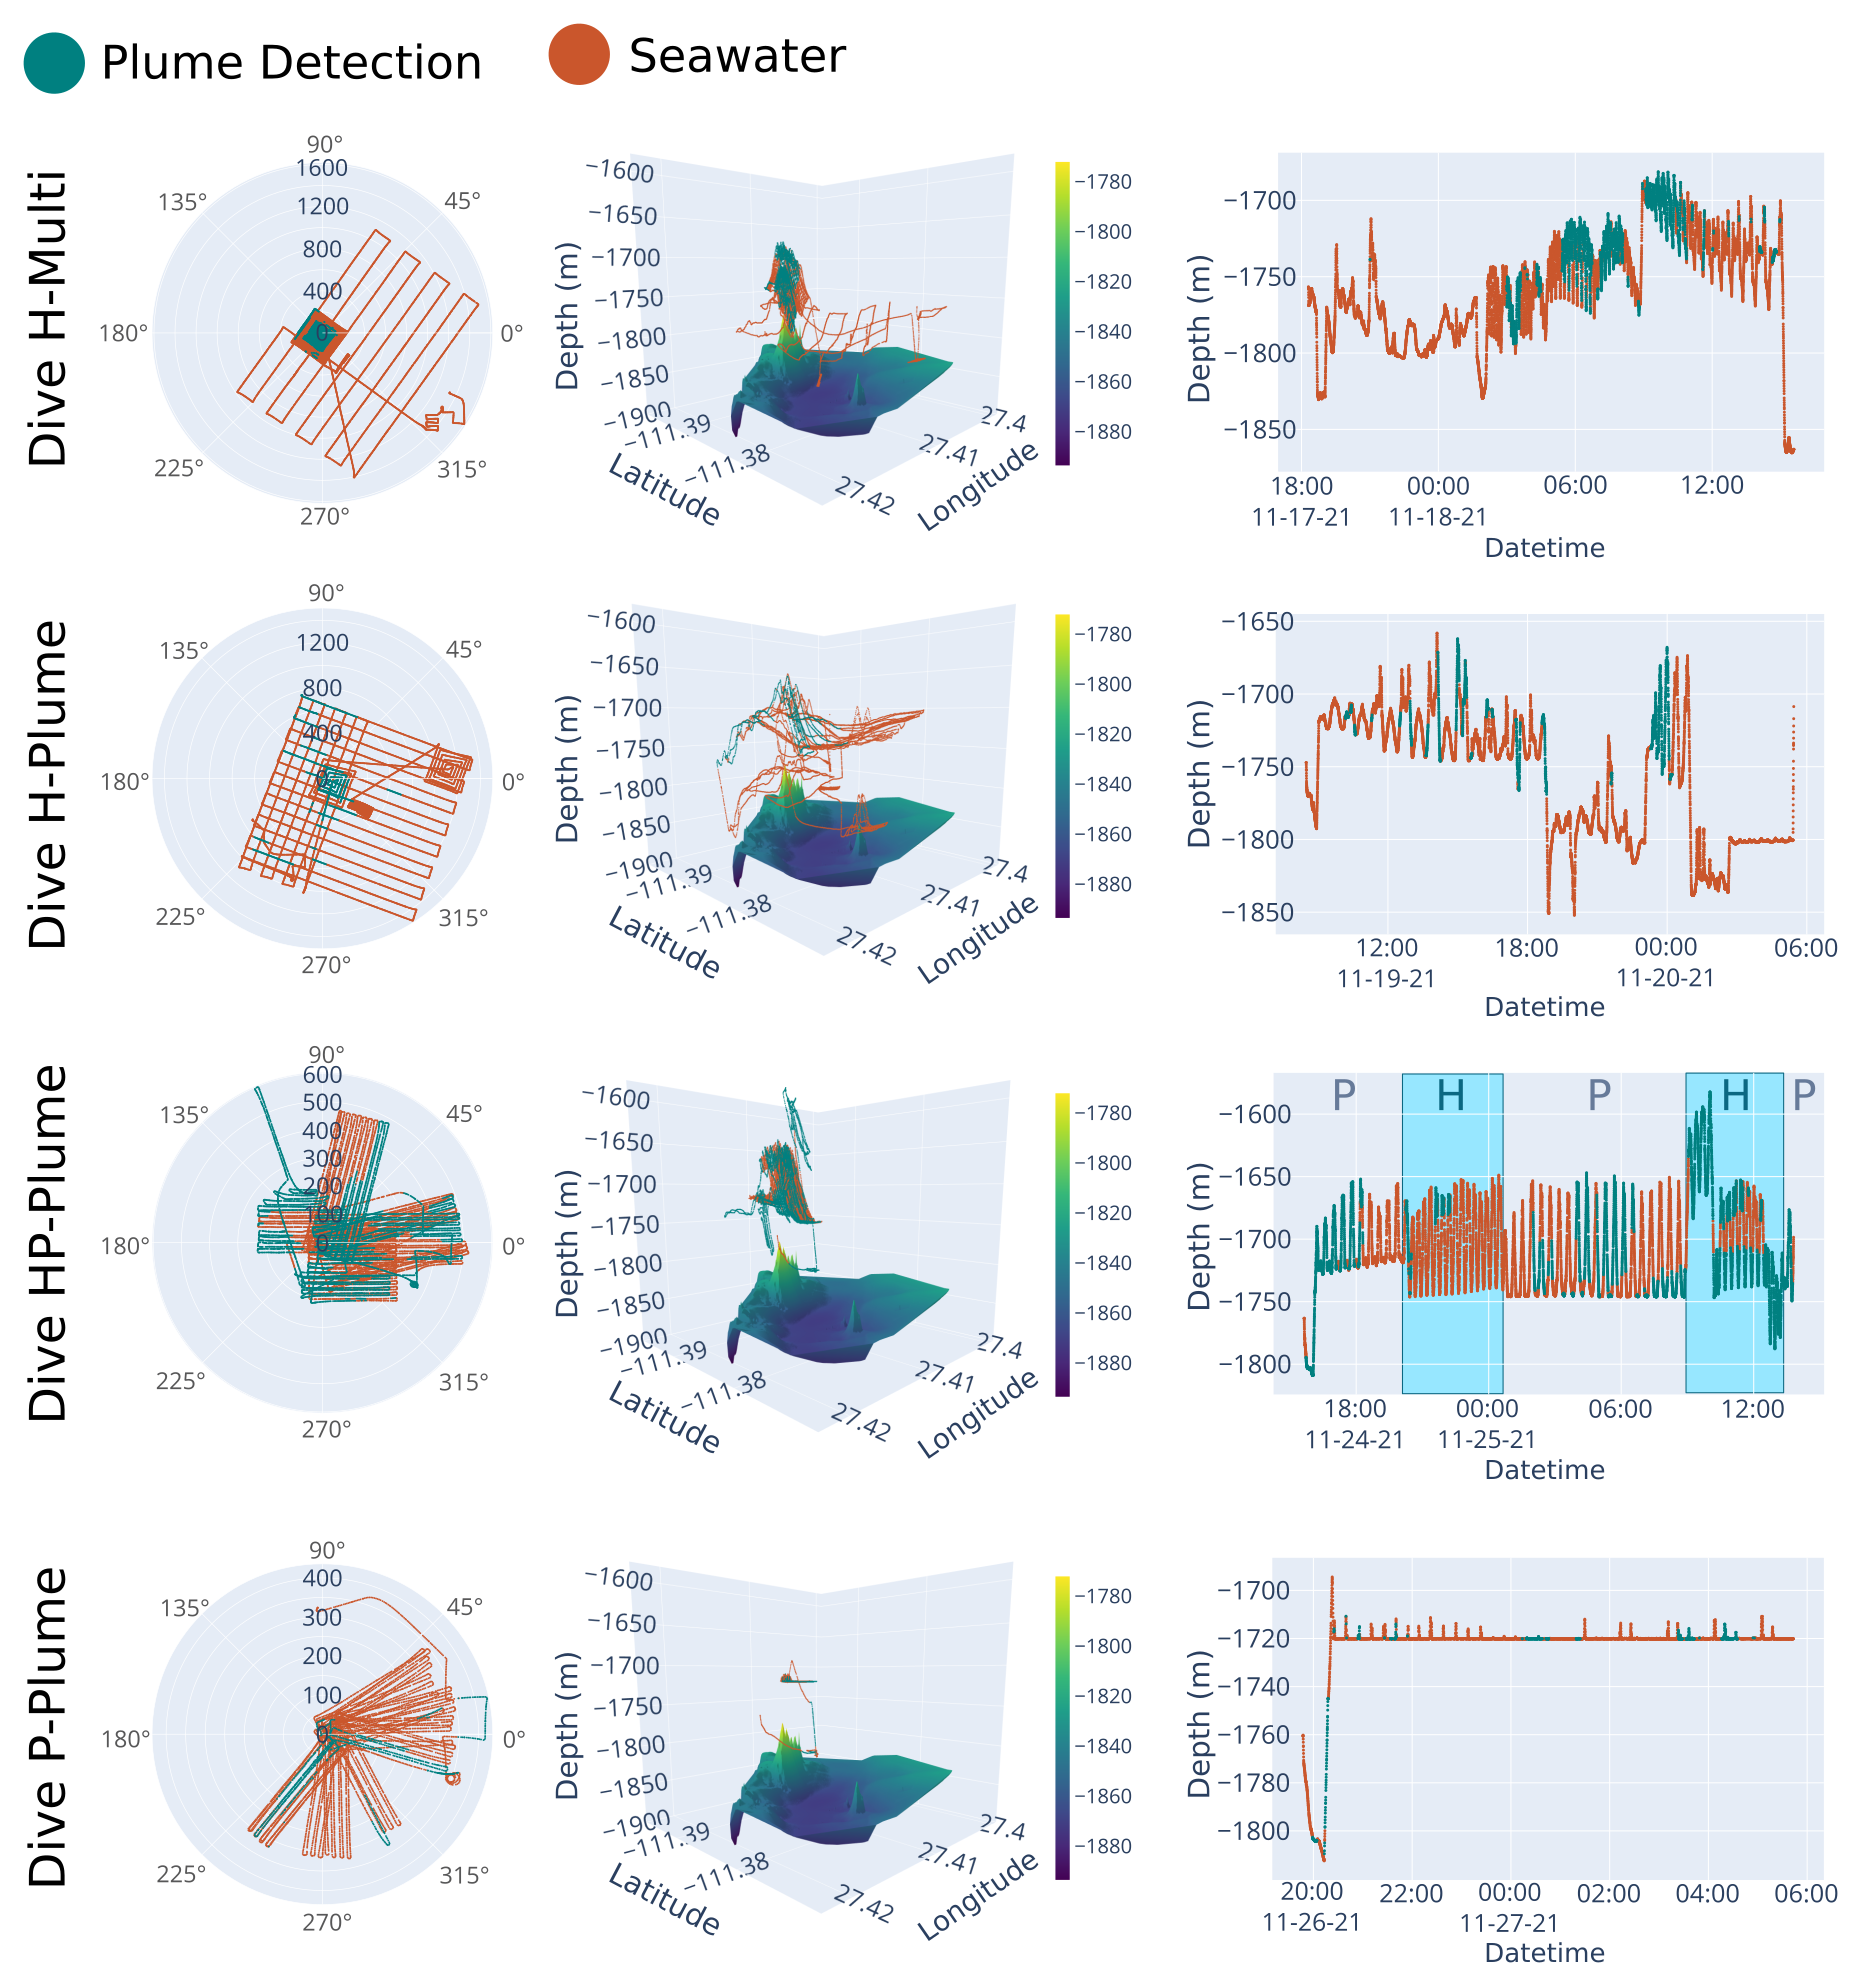
\includegraphics[width=1.0\columnwidth]{figures/detections_data.png}
    \caption{\textbf{The four field dives of AUV \Sentry.} All data is plotted according to its detection identity (in-plume or seawater). The first column shows a top-view of the dive trajectories in polar coordinates, in which angle and radius is computed relative to the chimney coordinate of the vent of study. In the center column, the 3D path of the vehicle over the rendered bathymetric terrain is provided. All but Dive P-Plume were dives conducted in altitude-hold mode with \Sentry, and so the trajectories show obvious changes in elevation; in contrast Dive P-Plume was held in depth-hold mode, so most observations are gathered within a depth-plane. The final column shows a time series versus depth of the detections collected. In Dive HP-Plume the portions of the dive that were human-designed and \PHORTEX-designed are labeled with H and P, respectively. As can be seen in the Dive HP-Plume time series, the two human-designed trajectories have significantly different performance, despite being in locally similar regions of the spatial domain. }
    \label{fig:field_results}
\end{figure}

In this field deployment, we demonstrate that \PHORTEX is a useful and practical tool for plume-charting. The performance of trajectories designed with \PHORTEX are comparable to those designed by human experts with key improvements in spatial and temporal utilization. It is further worth highlighting that \PHORTEX was trained only on data collected during the first dive, H-Multi, and reasonable performance during P-Plume using week-old training data emphasizes the long-range forecasting ability of the approach. Practically, the automated nature of \PHORTEX operationally alleviates significant decision-making burden on a science team and the trajectory-design burden on the \Sentry team; the ability to ingest data from external sensors and previous \Sentry missions, and produce trajectories that can be seamlessly ingested by the safety checking system without human intervention is of considerable benefit in the field. Moreover, the intermediate products of \PHORTEX, such as \PHUMES forecasts, are useful for other tasks in field operations, such as deploying other instruments or prioritizing instrument deployment order based on temporal changes in the environment by virtue of yielding rich context easily interpretable by the science team. 

% Similarly, \PHORTEX is trained on significantly less data than what the human experts had access to throughout the cruise; this emphasizes the advantage of the model-based, data-aggregation approach in \PHUMES. 

\paragraph{\PHUMES Validation with Basin Observations}
While there is no external ``ground-truth'' that we can use to evaluate the performance of \PHORTEX, we can compare the \PHUMES model trained on external and binary \Sentry observations with snapshots of the vertical distribution of turbidity near the hydrothermal ridge to get a sense for the utility of the \PHUMES model. After training, \PHUMES estimated the fluid exit velocity from the target chimney to be \SI{0.58}{\meter\per\second}, the vent area to be \SI{0.82}{\meter\squared}, and the vertical and horizontal mixing coefficients to be 0.15 and 0.19, respectively. Simulating these conditions with an initial vent temperature of \SI{340}{\celsius} and salinity of 34.908 PSU under a nominal crossflow of \SI{0.11}{\meter\per\second}, we compare the time-averaged plume height and width with the turbid intrusion that is observed in vertical casts of a shipboard rosette. The rosette was lowered and raised through the water column using a cable and winch on the ship; several vertical transects were collected over the course of the research cruise at the target autonomy site in addition to other sites throughout the basin. In \cref{fig:field_valid} we show two vertical transects, one conducted about \SI{100}{\meter} from a known vent, and one conducted \SI{600}{\meter} from the same vent. We see that within the model regions for predicted plume intrusions in the water column, strong turbid signals are observed in both vertical transects. This is indicative that the learned \PHUMES model is capable of uncovering the structure of the hydrothermal plume and lends confidence that the model is informative for planning sample trajectories that will intersect with plume fluids.

\begin{figure}[h!]
    \centering
    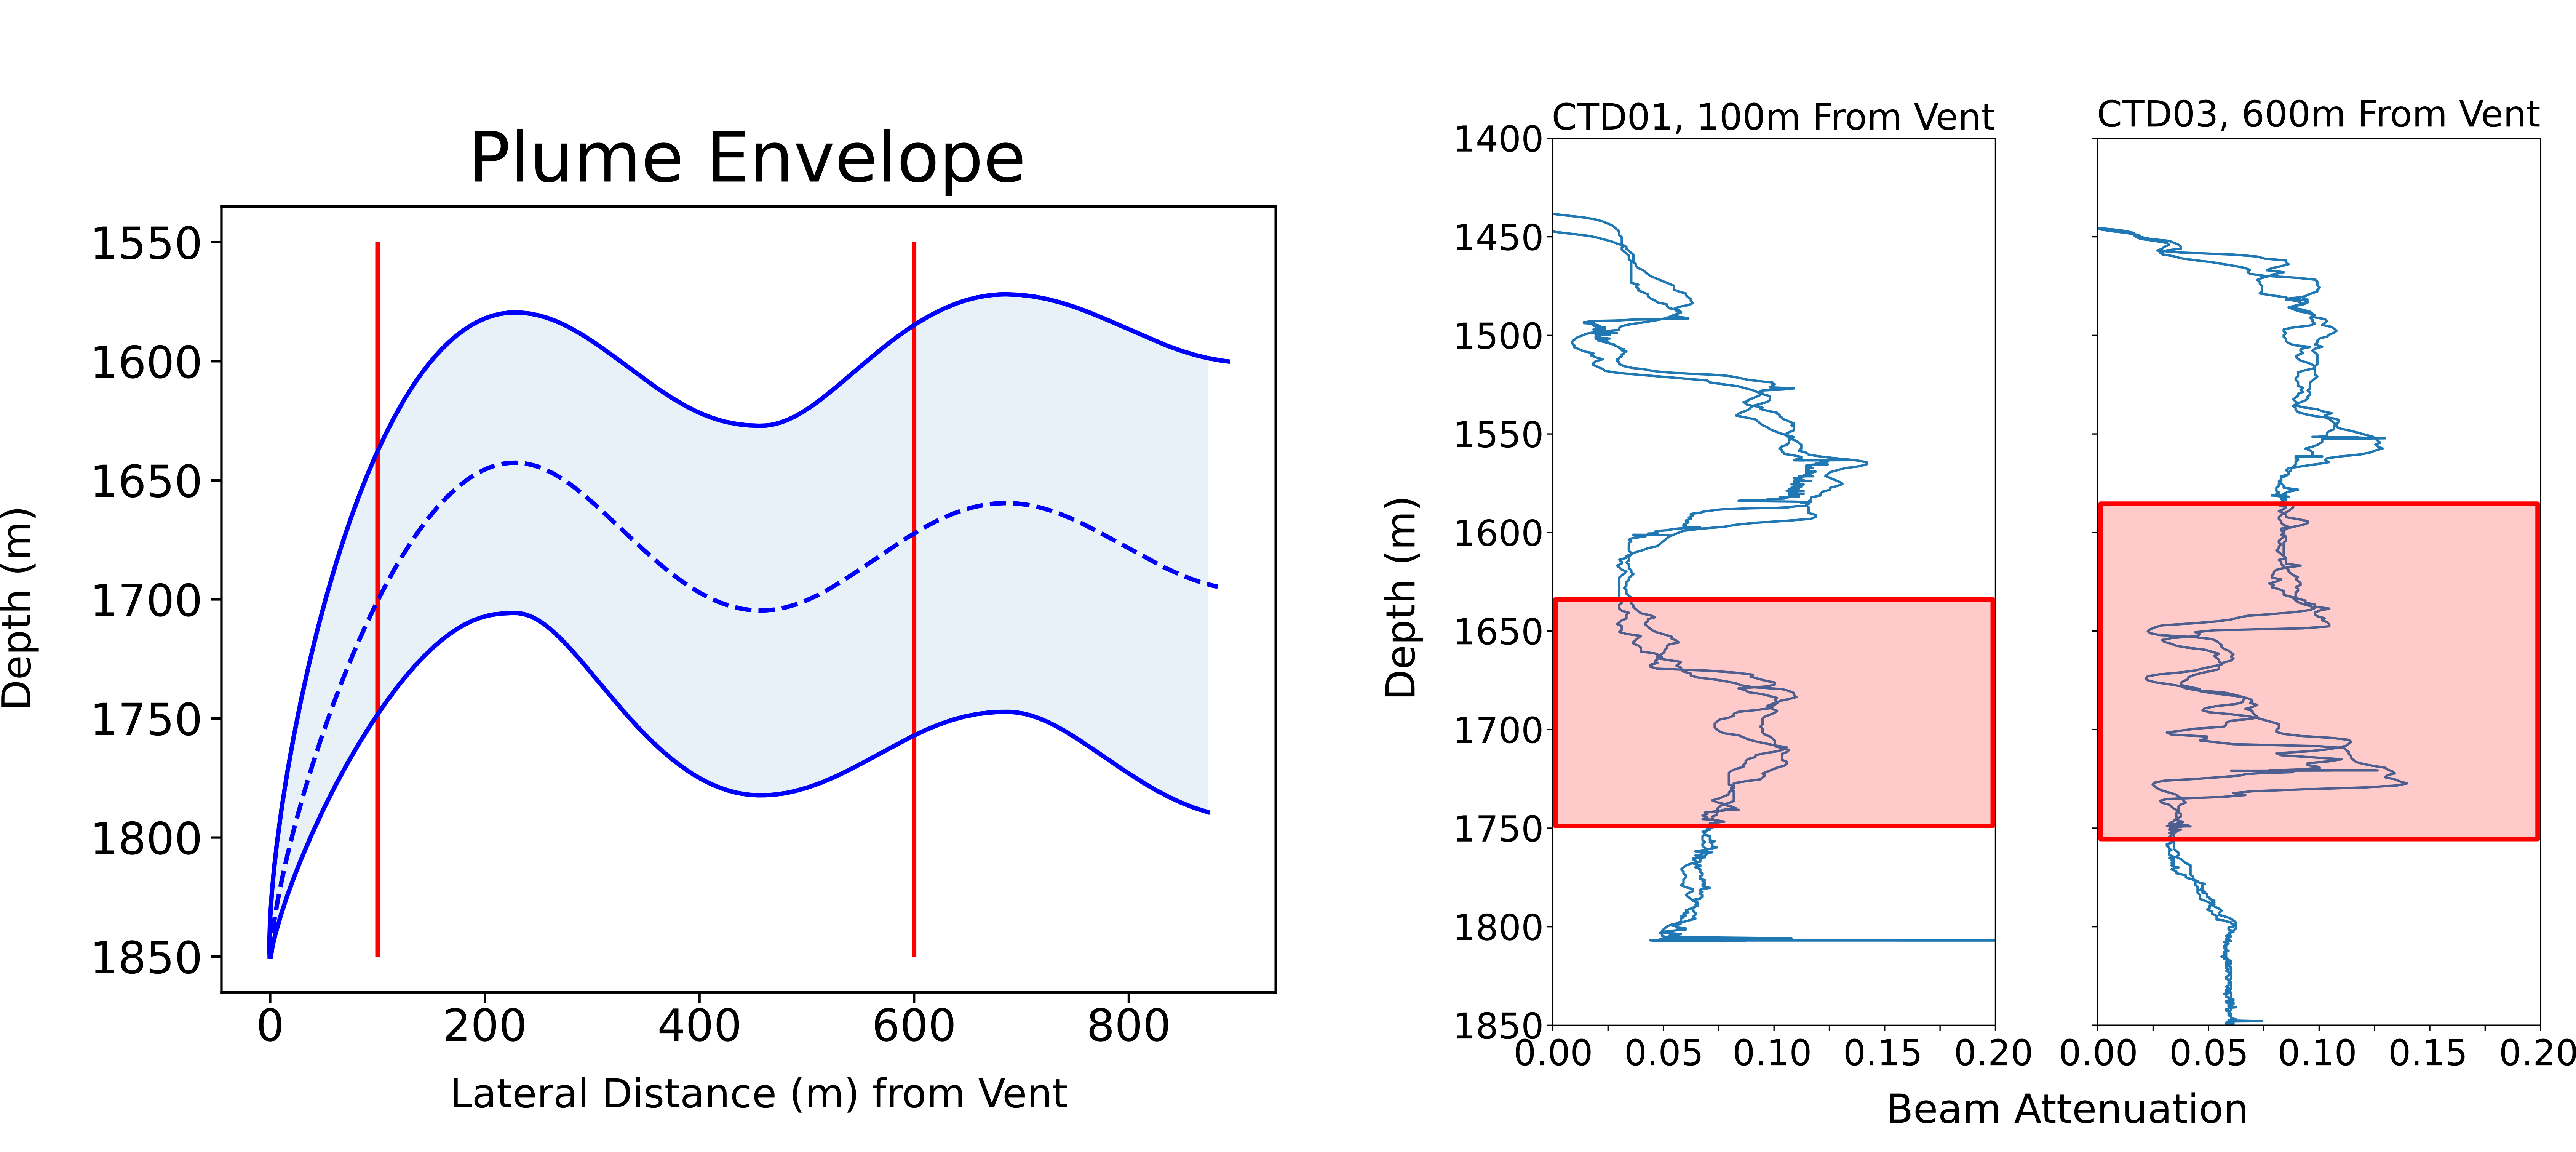
\includegraphics[width=1\columnwidth]{figures/field_validation.png}
    \caption{\textbf{Validation of \PHUMES model trained at sea.} We compare the nominal plume estimate from \PHUMES trained on at-sea data and \Sentry observations with vertical transects of turbidity from shipboard rosette. The plume envelope is the average plume estimated by \PHUMES for a nominal crossflow of \SI{0.12}{\meter\per\second}. Vertical red lines mark \SI{100}{\meter} and \SI{600}{\meter} laterally from the originating vent, for which vertical CTD casts were conducted. The region that the model estimates containing the lowest plume intrusion in the water column is highlighted on the turbidity transects. There is agreement between the model estimate and the transect data on the location of this turbid layer.} 
    \label{fig:field_valid}
\end{figure}


% \td{Note that this section is under construction! An overview of what this section will entail is below!}

% \begin{itemize}
%     \item This section will primarily present 4 trials that we performed while at sea -- 1 designed completely by hand, 2 partially designed by a person and by \PHORTEX, and one completely designed by \PHORTEX. The intent is to show the ``planning spectrum'' from fully-human to fully algorithmic, and comment on the form of these plans and their relative efficacy. Note that because the conditions between each iteration are different, the iterations are themselves not necessarily directly comparable (as in, claiming that one is ``better'' than another may be...bold) so we will be primarily focused on general metrics across all dives.
%     \item The Planning Spectrum: \begin{itemize}
%         \item We will show each of the 4 dives from fully human-designed to fully algorithmically designed. We will point out how the form factor between the lawnmowers/lawnmower chains differ, highlighting in particular how algorithmic chains tend to be strongly impacted by estimated crossflow, causing the trajectories to ``fan'' out; whereas human design trajectories tend to be conservatively placed centered at a known source.
%         \item We will show each of the four dives in both space and time; this will allow us to mark-up the figures and show where and when detections were made. We will ideally show that algorithmic trajectories tend to have more evenly distributed detections throughout a dive. We will also hopefully show that algorithmic trajectories tend to have more ``far afield'' positive detections of plumes.
%     \end{itemize}
%     \item Quantitative Results: \begin{itemize}
%         \item Some quantitative results we will share for each dive will include proportion of total samples in plume, proportion of total samples within/outside a certain radius from a known vent, RMSE of estimates vent characteristics by \PHUMES (train a naive \PHUMES model from observations collected by each dive, how to the dives inter-compare? How does it compare with estimates from ROV \emph{JASON}? How does a per-dive iteration look?)
%     \end{itemize}
% \end{itemize}

